\documentclass[10pt,b5paper,twoside]{book}

%\usepackage{algorithm}  
%\usepackage{algorithmic}  
\usepackage{wallpaper} %使用wallpaper宏包

\usepackage[final]{pdfpages} %插入整页pdf
\usepackage[T1]{fontenc}
\usepackage{CJKutf8}
%\usepackage{CJK}
\usepackage[utf8]{inputenc}
\usepackage{amsmath}
\usepackage{amsfonts}
\usepackage{amssymb}
\usepackage{subfigure}
\usepackage{graphicx}
\usepackage{grffile}
\usepackage{epstopdf}%支持eps格式图
\usepackage[centerlast]{caption}
% \counterwithin{figure}{section} %图按照章节编号
\counterwithin{figure}{chapter} %图按照章节编号
% \counterwithin{equation}{section} %公式按照章节编号
\counterwithin{equation}{chapter} %公式按照章节编号
\counterwithin{table}{section} %表按照章节编号
%\usepackage{fourier}
\usepackage[left=2cm,right=2cm,top=2cm,bottom=2cm]{geometry}

\usepackage[export]{adjustbox}
\graphicspath{ {./images/} }

%设置缩进
\usepackage{indentfirst} 
\setlength{\parindent}{2em}

%设置行距
\linespread{1.4}

%设置章节显示
\usepackage[center]{titlesec}
%\titleformat{\chapter}
\definecolor{gray75}{gray}{0.75}
\newcommand{\hsp}{\hspace{20pt}}
\titleformat{\chapter}{\Huge\bfseries}{\begin{CJK}{UTF8}{gkai}第\,\thechapter\,章\hsp\textcolor{gray75}{|}\hsp\end{CJK}}{0pt}{\Huge\bfseries}

\newcommand{\chap}[1]{\begin{CJK}{UTF8}{gkai}\chapter{#1} \end{CJK}}

\makeatletter %使\subsection中的内容左对齐
\renewcommand{\subsection}{\@startsection{subsection}{2}{0mm}
  {-\baselineskip}{0.5\baselineskip}{\bf\leftline}}
\renewcommand{\subsubsection}{\@startsection{subsubsection}{2}{0mm}
  {-\baselineskip}{0.5\baselineskip}{\bf\leftline}}

% 更改目录的章显示
\usepackage{titletoc}
\titlecontents{chapter}[0pt]{\addvspace{1.5pt}\filright\bf}%
               {\contentspush{第\,\thecontentslabel\,章\quad}}%
               {}{\titlerule*[8pt]{.}\contentspage}

% 更改页眉页脚为第几章形式
%\usepackage{fancyhdr}%导入fancyhdr包
%\pagestyle{fancy}
%\fancyhead{} % 初始化页眉
%\renewcommand{\chaptermark}[1]{\markboth{#1}{}}
\renewcommand{\chaptermark}[1]{\markboth{\begin{CJK}{UTF8}{gkai}第\,\thechapter\,章\, #1\end{CJK}}{}}
\renewcommand{\sectionmark}[1]{\markright{\thesection\, #1}}


%\fancyhead[LE]{\textsl{\rightmark}}
%\fancyhead[RO]{\textsl{\leftmark}}
%\renewcommand{\sectionmark}[1]{\markright{\thesection\,节\, #1}}
%\renewcommand{\chaptermark}[1]{\markright{第\,\thechapter\,章\, #1}{}}

%c++代码显示环境
\usepackage{listings}
\lstset{language=C++}

%算法伪代码环境
\usepackage[ruled,vlined]{algorithm2e}
%\usepackage[linesnumbered,lined,boxed,commentsnumbered]{algorithm2e}
%\usepackage{algorithm}
%\usepackage{algorithmic}

% 超链接设置及冲突解决
\usepackage{hyperref}
\hypersetup{unicode}
\hypersetup{colorlinks=true, linkcolor=blue, filecolor=magenta, urlcolor=cyan,}
\urlstyle{same}
%\hypersetup{CJKbookmarks=true}%让设置超链接后章节里面能写中文

%更改目录
\renewcommand{\contentsname}{目录}

% 更改算法显示为中文
\renewcommand{\algorithmcfname}{算法}

%更改图表的显示
\renewcommand{\figurename}{图}
\renewcommand{\tablename}{表}

\begin{document}
\begin{CJK}{UTF8}{gkai}

	\setcounter{page}{0}
	\pagenumbering{roman}
\begin{titlepage}
  \vspace*{1cm}
	\begin{center}
		{\Huge \textbf{计算机图形学中的四元数}\par}
		%{\large \textbf{第三册}\par}
		%{\Huge\raggedright 图形瑰宝\par}
  		%\noindent\hrulefill\par
  		\vspace*{1cm}
  		{\large\raggedleft John Vince  著\par}
  		{\large\raggedleft 郭飞  译\par}
  		
  		\vfill
  		{\Large 2023年\par}
  		%{\Large\raggedleft Institute\par}
	\end{center}
\end{titlepage} 
\thispagestyle{empty}
\begin{titlepage}
	\vspace*{5cm}
	\begin{center}
		\textit{谨以此书献给Heidi.} 
	\end{center}
\end{titlepage}
\thispagestyle{empty}
\clearpage
\mbox{}
\end{CJK}
%\begin{titlingpage}
%\maketitle
%\end{titlingpage}
%\includepdf{booktest (another copy).pdf}

%\newpage

%\maketitle

%\ThisCenterWallPaper{0.5}{./fig/cover.png}


\begin{CJK}{UTF8}{gbsn}
\newpage
\pdfbookmark{译序}{yixu}
\section*{译序} 
% \bookmark[dest=\HyperLocalCurrentHref, level=0]{译序}
%\bookmark[page=5,level=0]{译序}
% \pdfbookmark{译序}{section}
333

\newpage
\pdfbookmark{序}{xu}
\section*{序}

%\bookmark[page=6,level=0]{序}
% \bookmark[dest=\HyperLocalCurrentHref, level=0]{序}

50多年前,当我正在学习成为一名电气工程师时,我遇到了复数,它们被用来用$j$操作符表示异相电压和电流。我相信使用的是字母$j$,而不是$ i $,因为后者代表电流。因此,从我学习的一开始,我就在脑海中清晰地描绘了一个假想的单位,它是一个旋转算子,可以在时间上推进或延缓电量。


当事情决定我要从事计算机编程而不是电气工程的职业时,我不需要复数,直到Mandlebrot关于分形的工作出现。但那只是暂时的阶段,我从来都不需要在我的任何电脑图形软件中使用复数。然而在1986年,当我加入飞行模拟行业时,我看到了一份关于四元数的内部报告,它被用于控制模拟飞机的旋转方向。

我仍然记得我对四元数的困惑,仅仅是因为它们包含了很多虚数。然而,经过大量研究,我开始了解它们是什么,但不知道它们是如何工作的。与此同时,我对数学的哲学方面产生了兴趣,并试图通过伯特兰·罗素的著作来理解数学的“真正意义”。因此,像$i$这样的概念是一个智力挑战。

我现在对虚数$ i $不过是一个符号的想法感到满意,并且在代数的上下文中允许定义$ i ^{2}=-1$。我相信,试图发现它存在的更深层次的意义是徒劳的。尽管如此,它在数学中是一个令人惊叹的对象,我经常想是否会有类似的对象等待被发明出来。

当我开始写关于计算机图形学的数学书籍时,我学习了复分析,以便有信心地写复数。就在那时,我发现了向量和四元数发明背后的历史事件,主要是通过Michael Crowe的优秀著作《向量分析的历史\footnote{ A History of Vector Analysis}》。这本书让我认识到理解数学发明如何以及为什么发生的重要性。


最近,我读到了Simon Altmann的书《旋转、四元数和双群\footnote{Rotations, Quaternions, and Double Groups} 》,这本书提供了关于十九世纪四元数消亡\footnote{demise,感觉不应该译为消亡}的进一步信息。Altmann非常热衷于确保Olinde Rodrigues的数学工作得到认可,后者发表了一个与汉密尔顿四元数生成的公式非常相似的公式。罗德里格斯发表论文的一个重要方面是,它比汉密尔顿在1843年发明四元数早了三年。然而,罗德里格斯并没有发明四元数代数——这个奖必须颁给汉密尔顿——但他确实理解三角函数中半角的重要性,三角函数用于围绕任意轴旋转点。

任何使用过欧拉变换的人都会意识到它的缺点,尤其是它的阿喀琉斯之踵:万向节锁。因此,任何可以围绕任意轴旋转点的设备都是程序员工具包中受欢迎的补充。在平面和空间中有许多旋转点和帧的技术,我在我的书《计算机图形的旋转变换\footnote{Rotation Transforms for Computer Graphics}》中详细介绍了这些技术。那本书还涵盖了欧拉-罗德里格斯参数化和四元数,但只是在提交了手稿准备出版之后,我才决定写这本专门关于四元数的书,以及它们是如何和为什么被发明的,以及它们在计算机图形学中的应用。

在研究这本书的同时,阅读William Rowan Hamilton和他的朋友P.G. Tait的一些早期书籍和论文非常有启发性。我现在明白了完全理解四元数的意义是多么困难,以及如何利用它们。当时,没有围绕任意轴旋转点的主要需求;然而,需要一个数学系统来处理矢量。最后,四元数不再是当月的宠儿,慢慢地淡出了人们的视线。尽管如此,能够表示向量并对它们进行算术操作是汉密尔顿的一个重大成就,尽管乔赛亚·吉布斯(Josiah Gibbs)有远见地创建了一个简单可行的代数框架。

在这本书中,我试图描述一些围绕四元数发明的历史,以及对四元数代数的描述。我绝不认为自己是四元数方面的权威。我只是想谈谈我是如何理解它们的,希望对你们有用。四元数有不同的表示方式,但我最喜欢的是有序对,这是我在Simon Altmann的书中发现的。

这本书分为八章。第一章和最后一章是对本书的介绍和总结,共六章,内容包括以下主题。关于数集和代数的第二章回顾了与本书其余部分相关的符号和语言。有关于数集、公理、有序对、群、环和域的章节。这为读者准备了非交换四元数积,以及为什么四元数被描述为除法环。

第三章回顾了复数,并展示了复数如何表示为有序对和矩阵。第四章继续这一主题,介绍了复平面,并展示了复数的旋转特征。它还为读者准备了一个在19世纪早期提出的问题:是否有一个相当于复数的$3 D$ ?

第五章通过描述汉密尔顿的发明来回答这个问题:四元数及其相关代数。我在书中加入了一些历史信息,以便读者了解Hamilton著作的重要性。虽然有序对是表示法的主要形式,但我也包括了矩阵表示法。

为了让读者了解四元数的旋转特性,第6章回顾了3D旋转变换,特别是欧拉角和万向节锁。我还开发了一个矩阵,用于使用向量和矩阵变换围绕任意轴旋转一个点。

第7章是本书的重点,描述了四元数如何围绕任意轴旋转向量。本章以一些历史信息开始,并解释了不同的四元数乘积如何旋转点。虽然四元数很容易使用它们的复杂形式或有序对符号来实现,但它们也有一个矩阵形式,这是从第一性原理发展而来的。本章继续讨论特征值、特征向量、围绕偏移轴旋转、旋转参照系、插值四元数以及四元数和旋转矩阵之间的转换。

每一章都有很多实际的例子来说明如何计算方程,每章末尾会给出进一步的例子。

写这本书是一段非常愉快的经历,我相信你也会喜欢读它,并从书中发现一些新的东西。

我要感谢米德尔塞克斯大学荣誉读者Tony Crilly博士,他阅读了一份手稿草稿,并纠正和澄清了我的注释和解释。托尼在我的书《计算机图形的旋转变换》中执行了相同的任务。我绝对信任他的数学知识,我感谢他的建议和专业知识。然而,我仍然为我可能犯的任何代数错误承担全部责任。

我还要感谢Patrick Riley教授,他阅读了手稿的一些早期草稿,并提出了一些关于四元数的有趣技术问题。这样的问题让我意识到我对四元数的一些描述需要进一步澄清,希望这些描述已经得到纠正。

我现在已经在我的三本书中使用了\LaTeX$ 2\varepsilon$ ,并且对它的符号有了信心。尽管如此,我仍然需要致电施普林格的技术支持团队,感谢他们的帮助。

我不确定这是否是我的最后一本书。如果是的话,我要感谢贝弗利·福特,计算机科学的编辑主任,和海伦·德斯蒙德,施普林格英国计算机科学的副主编,他们在过去几年的专业支持。如果这不是我的最后一本书,那么我期待着在另一个项目上与他们再次合作。


Ringwood, UK  \hfill                                               John Vince

\tableofcontents

\newpage
\setcounter{page}{0}
\pagenumbering{arabic}

\chap{介绍}
\section{旋转变换}
在计算机图形学中,我们使用变换来修改对象或虚拟摄像机的位置和方向。这种变换通常包括:缩放、平移和旋转。前两个变换很简单,但是旋转确实会引起问题。这是因为我们通常从围绕$x-, y$ -和$z$-轴的单独旋转中构造一个旋转变换。尽管这样的转变行之有效,但还远远不够完美。真正需要的是一种直观、简单和准确的技术。

多年来,旋转变换包括方向余弦,欧拉角,欧拉-罗德里格斯参数化,四元数和多向量。最后两种技术是最新的,并且与历史相关。然而,这本书的主题是四元数,以及它们如何在计算机图形学中使用。


\section{目标读者}
这本书的目标读者学习或工作在计算机图形学和需要一个四元数的概述。他们可能就是我在互联网论坛上遇到过的询问四元数、它们如何工作以及如何编码的人。希望这本书能回答大部分问题。


\section{本书的宗旨和目标}
这本书的主要目的是向读者介绍四元数的主题,以及它们如何用于围绕任意轴旋转点。第二个目标是让读者意识到所有数学发现背后的人的层面。就我个人而言,我认为我们绝不能忽视这样一个事实:数学家也是人。尽管他们可能被赋予了非凡的数学技能,但他们恋爱、结婚、成家、死亡,留下了一座令人惊叹的知识大厦,我们都从中受益。

鼓励那些对数学的人类维度感兴趣的读者阅读四元数的发明,并发现爱、兴趣、坚韧、灵感和奉献是如何导致一项重大数学发现的。迈克尔·克罗的《矢量分析的历史》[10]是一本必不可少的书。这提供了导致四元数发明的事件的彻底分析,以及向量分析的出现。第二本书是Simon Altmann的《旋转、四元数和双群[1]》,除了提供了四元数代数的现代分析外,还介绍了Olinde Rodrigues,他比通常被公认为四元数之父的William Rowan Hamilton早三年发明了一些与四元数相关的数学。

Simon Altmann对四元数代数的分析对我自己对四元数的看法产生了深远的影响,我试图在接下来的章节中传达这一点。特别地,我采用了使用有序对来表示四元数的思想。

本书的首要目标是使读者能够设计和编码四元数算法。读完这本书后,这应该是一个简单的练习,尽管我们处理的是一个四维数学对象。

\section{数学技术}
一旦读者理解了四元数,就会认为它们很简单。然而,如果这是你第一次遇到他们,他们可能会显得很奇怪。但像所有事物一样,熟悉带来理解和信心。

为了描述四元数,我需要用到一点三角学,一些向量理论和矩阵代数。由于四元数被描述为“超复数”,因此有一章是关于复数的。


\section{本书中的假设}
很多时候,从事计算机图形工作的人——比如我自己——没有机会学习技术文献中经常使用的数学水平。因此,我故意在写这本书的时候,温和地介绍了从复杂代数到四元数代数的形式数学符号。
\chap{数集与代数}
\section{介绍}
在本章中,我们将回顾数集的一些基本思想,以及如何用算术和代数方法处理它们。我们简要地看一下表达式和方程,以及用于构造和求值的规则。这些反过来又揭示了用所谓的复数扩展日常数字的需要。

本章的第二部分用于定义组、环和域。

\section{数集}
\subsection{自然数}
自然数是整数1,2,3,4等,根据定义(DIN 5473),自然数的集合和零$\{0,1,2,3,4,\ldots\}$由符号$\mathbb{N}$表示,我们使用:
$$
\mathbb{N}=\{0,1,2,3,4, \ldots\} .
$$
该语句
$$
k \in \mathbb{N}
$$
意味着$k$属于集合$\mathbb{N}$,其中$\in$表示属于,或者换句话说,$k$是一个自然数。我们在本书中使用这种符号,以确保对所使用的数值量的类型没有混淆。

$ \mathbb {N} ^{*}$用于表示集合$\{1,2,3,4,\ldots \} $。

\subsection{实数}
科学计算使用大量的数学对象,如标量、向量和矩阵。标量只有一个数值,而矢量有两个或两个以上的数字来编码矢量的大小和方向。矩阵是一个矩形数组的数字,可能有各种各样的属性。

十进制数构成由$\mathbb{R}$标识的实数集。这样的数字是有符号的,可以组织成一条线,延伸到$-\infty$和$+\infty$,其中包括0。无限的概念很奇怪,德国数学家康托(Georg Cantor, 1845-1918)研究过这个概念。康托尔还发明了集合论,证明了实数比自然数多。幸运的是,我们不需要在本书中使用这些概念。

\subsection{整数}
整数集$\mathbb{Z}$包含自然数及其负数:
$$
\mathbb{Z}=\{\ldots,-3,-2,-1,0,1,2,3, \ldots\} .
$$
$\mathbb{Z}$代表zahlen——德语“数字”的意思。


\subsection{有理数}
有理数的集合是$\mathbb{Q}$,包含如下形式的数:
$$
\frac{a}{b}
$$
其中 $a, b \in \mathbb{Z}$ 且 $b \neq 0$.

\section{算术运算}
我们使用加法、减法、乘法和除法运算来操作数字,其结果是闭的还是不闭的,或者是未定义的,这取决于底层集合。例如,当我们将两个自然数相加时,结果总是另一个自然数,因此,运算是封闭的:
$$
3+4=7 .
$$
然而,当我们减去两个自然数时,结果不一定是一个自然数。例如,尽管
$$
6-2=4
$$
是一个封闭的操作,
$$
2-6=-4
$$
不是封闭的,因为$-4$不是自然数集合中的一员。两个自然数的乘积通常是一个封闭的运算,但是除法会引起一些问题。首先,将一个偶数除以2是一个封闭运算:
$$
16 / 2=8 .
$$
然而,将一个奇数自然数除以一个偶数自然数得到一个十进制数:
$$
7 / 2=3.5
$$
并且不封闭,因为$3.5$不属于自然数集合。这是用集合语言写的
$$
3.5 \notin \mathbb{N}
$$
其中 $\notin$ 表示不属于.

将任何数字乘以零都得到零——这是一个封闭运算;然而,任何数字除以零都是没有定义的,必须排除。

实数没有任何与自然数相关的问题,并且在加法、乘法和除法上有闭包:
$$
\begin{aligned}
a+b & =c & & a, b, c \in \mathbb{R} \\
a b & =c & & a, b, c \in \mathbb{R} \\
a / b & =c & & a, b, c \in \mathbb{R} \text { and } b \neq 0 .
\end{aligned}
$$
注意,$a b$是$a \times b$的简写。


\section{公理}
当我们构造代数表达式时,我们使用称为公理的特定定律。对于加法和乘法,我们知道数字的分组对最终结果没有影响:例如$2+(4+6)=(2+4)+6$和$2 \times(3 \times 4)=$ $(2 \times 3) \times 4$。这是结合律公理,表示为:
$$
\begin{aligned}
a+(b+c) & =(a+b)+c \\
a(b c) & =(a b) c .
\end{aligned}
$$
我们也知道,当加或乘时,顺序对最终结果没有影响:例如$2+6=6+2$和$2 \times6=6 \times2$。这是交换公理,表示为:
$$
\begin{aligned}
a+b & =b+a \\
a b & =b a .
\end{aligned}
$$
代数表达式包含各种各样的乘积,涉及一个实数和一串实数,它们服从分配律:
$$
\begin{aligned}
a(b+c) & =a b+a c \\
(a+b)(c+d) & =a c+a d+b c+b d .
\end{aligned}
$$
我们回顾这些公理的原因是,它们不应该被视为刻在数学石头上的,而适用于所有被发明的东西。因为当我们讲到四元数时,我们会发现它们不遵守交换公理,这并不奇怪。如果你用过矩阵,你就会知道矩阵乘法也是不可交换的,但是是结合的。
\section{表达式}
使用上述公理,我们能够构造各种表达式,例如:
$$
\begin{aligned}
& a(2+c)-d / e+a-10 \\
& g /(a c-b d)+h /(d e-f g) .
\end{aligned}
$$
我们还使用符号来提高一个量的幂,如$n^{2}$。这个符号引入了另一组观察结果:
$$
\begin{aligned}
a^{n} a^{m} & =a^{n+m} \\
\frac{a^{n}}{a^{m}} & =a^{n-m} \\
\left(a^{n}\right)^{m} & =a^{n m} \\
\frac{a^{n}}{a^{n}} & =a^{0}=1 \\
\frac{1}{a^{n}} & =a^{-1} \\
a^{1 / n} & =\sqrt[n]{a} .
\end{aligned}
$$
接下来,我们必须包括各种各样的函数,比如平方根、正弦和余弦,这些函数看起来相当简单。但我们必须警惕他们。例如,按惯例,$\sqrt{16}=4$。但是,$x^{2}=16$有两个解:$\pm \sqrt{16}=\pm 4$。然而,$\sqrt{-16}$不存在自然数或实数解。因此,如果$a<0$,表达式$\sqrt{a}$就没有实根。

类似地,在处理正弦和余弦等三角函数时,我们必须记住,这些函数的值范围在$-1$和$+1$之间,包括0,这意味着如果将它们用作分母,结果可能是未定义的。例如,如果$\sin \alpha=0$,则此表达式未定义
$$
\frac{a}{\sin \alpha} \text {. }
$$

\section{等式}
接下来,我们来到方程,我们将表达式的值赋给变量。在大多数情况下,任务是直接的,并导致一个真实的结果,如
$$
x^{2}-16=0
$$
其中$x=\pm 4$。但有趣的是,只要把符号颠倒过来
$$
x^{2}+16=0
$$
我们创建了一个没有实解的方程。然而,有一个复杂的解决方案,这是第三章的主题。

\section{有序对}
$(a, b)$是一个有两个坐标或投影项的对象,其中第一个或左边的项与第二个或右边的项是不同的。例如,$(a, b)$与$(b, a)$是不同的,除非$a=b$。也许有序对的最好例子是$(x, y)$,它表示平面上的一个点,其中元素的顺序总是$x$-坐标后面跟着$y$-坐标。

在计算机图形学中,有序对和有序三元组被广泛用于表示平面上的点$(x, y)$,空间中的点$(x, y, z)$,以及诸如$(r, g, b)$和$(h, s, v)$等颜色值。在这些例子中,字段都是实值。没有什么可以阻止我们使用有序对来开发一个代数,它的行为就像另一个代数一样,我们将在第三章对复数和第五章对四元数这样做。现在,让我们探索一些可以操纵有序对的方法。

假设我们选择将一个通用的有序对描述为
$$
a=\left(a_{1}, a_{2}\right) \quad a_{1}, a_{2} \in \mathbb{R} .
$$
我们将定义两个对象的加法为
$$
\begin{aligned}
a & =\left(a_{1}, a_{2}\right) \\
b & =\left(b_{1}, b_{2}\right) \\
a+b & =\left(a_{1}+b_{1}, a_{2}+b_{2}\right) .
\end{aligned}
$$
举例:
$$
\begin{aligned}
a & =(2,3) \\
b & =(4,5) \\
a+b & =(6,8) .
\end{aligned}
$$
我们将乘积定义为
$$
a b=\left(a_{1} b_{1}, a_{2} b_{2}\right)
$$
使用上面的值,结果是什么
$$
a b=(8,15) .
$$
记住,我们说了算,规则是我们定的。

另一个规则将控制有序对如何响应标量乘法。例如:
$$
\begin{aligned}
\lambda\left(a_{1}, a_{2}\right) & =\left(\lambda a_{1}, \lambda a_{2}\right) \quad \lambda \in \mathbb{R} \\
3(2,3) & =(6,9) .
\end{aligned}
$$
有了上面的规则,我们就可以写了
$$
\begin{aligned}
\left(a_{1}, a_{2}\right) & =\left(a_{1}, 0\right)+\left(0, a_{2}\right) \\
& =a_{1}(1,0)+a_{2}(0,1)
\end{aligned}
$$
如果我们用乘法法则对$(1,0)$和$(0,1)$进行平方,我们得到
$$
\begin{aligned}
& (1,0)^{2}=(1,0) \\
& (0,1)^{2}=(0,1)
\end{aligned}
$$
这表明它们表现得像实数,这并不出人意料。

这似乎不是很有用,但是等着看在复数和四元数的上下文中会发生什么。

\section{群,环,域}
数学家们使用一系列令人眼花缭乱的名字来识别他们的发明,这些发明似乎每天都在出现。甚至“四元数”这个名字也不是原创的,在历史上经常出现在“士兵的四元数”的语境中:

“罗马人派出四人组或四人组成夜间警卫……”[19]。

在不太正式的情况下,让我们探索更多与本书所包含的思想相关的数学结构。

\subsection{群}
我们已经讨论了集合的概念,以及属于集合意味着什么。我们还发现,当我们对集合的成员应用某些算术运算时,我们可以确保闭包、非闭包或结果未定义。

当将集合与算术运算结合在一起时,可以方便地创建另一个实体:群,即集合,以及描述集合元素如何组合的公理。集合可能包含数字、矩阵、向量、四元数、多项式等,并在下面表示为$a,b$和$c$。

公理使用'$o$'符号来表示任何二进制操作,如$+,-, \times$。一个群是由一个集合和一个二元运算组成的。例如,我们可能希望在加法下形成一组整数:$(\mathbb{Z},+)$,或者我们可能希望检查四元数是否在乘法操作下形成一组:$(\mathbb{H}, \times)$。

要成为一个群,对于集合$S$,所有下列公理必须成立。特别地,在中必须存在一个特殊的单位元素$e \in S$,并且对于每一个$a \in S$,在中必须存在一个逆元素$a^{-1} \in S$,从而满足下列公理:

\begin{align*}
    \begin{aligned}
        & \textbf{闭合: }        && a \circ b \in S && a,b \in S.\\
        & \textbf{结合律: }  && (a \circ b) \circ c=a \circ(b \circ c) && a, b, c \in S.\\
        & \textbf{单位元:}    && a \circ e=e \circ a=a && a, e \in S.\\
        & \textbf{可逆元素: }    && a  \circ a^{-1}=a^{-1} \circ a=e && a, a^{-1}, e \in S.
    \end{aligned}
\end{align*}
我们将一个组描述为$(S, \circ)$,其中$S$是集合,' 0 '是操作。例如$(\mathbb{Z},+)$是一组进行加法运算的整数,$(\mathbb{R}, \times)$是一组进行乘法运算的实数。

让我们通过三个例子将这些公理生动地展现出来。

$(\mathbb{Z},+)$:整数$\mathbb{Z}$在加法运算下形成一个组:
$$
\begin{aligned}
\text { 闭合: } & -23+24=1 \\
\text { 结合律: } & (2+3)+4=2+(3+4)=9 \\
\text { 单位元: } & 2+0=0+2=2 \\
\text { 可逆: } & 2+(-2)=(-2)+2=0 .
\end{aligned}
$$
$(\mathbb{Z}, \times)$:整数$\mathbb{Z}$在乘法下不构成群:
$$
\begin{aligned}
\text { 闭合: } & -2 \times 4=-8 \\
\text { 结合律: } & (2 \times 3) \times 4=2 \times(3 \times 4)=24 \\
\text { 单位元: } & 2 \times 1=1 \times 2=2 \\
\text { 可逆性: } & 2^{-1}=0.5 \quad(0.5 \notin \mathbb{Z}) .
\end{aligned}
$$
并且,整数0没有逆。

$(\mathbb{Q}, \times)$:非零有理数在乘法下构成一个群:
$$
\begin{aligned}
\text { 闭合: } & \frac{2}{5} \times \frac{2}{3}=\frac{4}{15} \\
\text { 交换律: } & \left(\frac{2}{5} \times \frac{2}{3}\right) \times \frac{1}{2}=\frac{2}{5} \times\left(\frac{2}{3} \times \frac{1}{2}\right)=\frac{2}{15} \\
\text { 单位元: } & \frac{2}{3} \times \frac{1}{1}=\frac{1}{1} \times \frac{2}{3}=\frac{2}{3} \\
\text { 可逆性: } & \frac{2}{3} \times \frac{3}{2}=\frac{1}{1} \quad\left(\text { where } \frac{3}{2}=\left(\frac{2}{3}\right)^{-1}\right)
\end{aligned}
$$

\subsection{阿贝尔群}
最后,以挪威数学家Neils Henrik Abel(1802-1829)的名字命名的阿贝尔群,是一个元素的顺序不影响结果的群,即群是可交换的。因此有五个公理:闭合性、结合性、单位元、逆元和交换性:
$$
\textbf{Commutativity:} \qquad a \circ b=b \circ a \qquad a, b \in S
$$
例如,整数集在普通加法$(\mathbb{Z},+)$下形成一个阿贝尔群。然而,由于三维旋转一般不交换,三维空间中所有旋转的集合形成了一个非交换群。

\subsection{环}
环是一个扩展的群,在这里我们有一组可以相加和相乘的对象,遵循一些精确的公理。有实数圈、复数圈、整数圈、矩阵圈、方程圈、多项式圈等。环被正式定义为一个系统,其中$(S,+)$和$(S, \times)$为阿贝尔群,分配公理如下:
$$
\begin{array}{lll}
\textbf { 加法结合律: } & a+(b+c)=(a+b)+c & a, b, c \in S . \\
\textbf { 乘法结合律: } & a \times(b \times c)=(a \times b) \times c & a, b, c \in S . \\
\textbf { 分配律: } & a \times(b+c)=(a \times b)+(a \times c) & \text { 和 } \\
& (a+b) \times c=(a \times c)+(b \times c) & a, b, c \in S .
\end{array}
$$
例如,我们已经知道整数$\mathbb{Z}$在加法运算下形成了一个群,但它们也形成了一个环,因为集合满足上述公理:
$$
\begin{aligned}
& 2 \times(3 \times 4)=(2 \times 3) \times 4 \\
& 2 \times(3+4)=(2 \times 3)+(2 \times 4) \\
& (2+3) \times 4=(2 \times 4)+(3 \times 4) .
\end{aligned}
$$

\subsection{域}
虽然环支持加法和乘法,但它们不一定支持除法。然而,由于除法是如此重要的算术运算,因此创建域是为了支持除法,但有一个限制条件:不允许除0。这样我们就有了实数$\mathbb{R}$、有理数$\mathbb{Q}$以及复数$\mathbb{C}$的域。然而,我们将发现四元数不构成域,但它们确实形成了所谓的除法环。

因此,每个域都是一个环,但并不是每个环都是一个场。

\subsection{除法环}
除法环或除法代数是一个环,其中每个元素都有一个逆元素,前提是该元素非零。代数也支持非交换乘法。下面是除法环$(S,+, \times)$的正式描述:
\begin{align*}
    \begin{aligned}
        &\textbf{加法结合律: } & (a+b)+c=a+(b+c) && a, b, c \in S \\
        &\textbf{加法交换律: } & a+b=b+a && a, b \in S\\
        &\textbf{加法单位元0 :}    & 0+a=a+0 && a, 0 \in S\\
        &\textbf{加法可逆性: }       & a+(-a)=(-a)+a=0 && a,-a \in S\\
        &\textbf{乘法结合律:} & (a \times b) \times c=a \times(b \times c) && a, b, c \in S\\
        &\textbf{乘法单位元 1:} &1 \times a=a \times 1 && a, 1 \in S\\
        &\textbf{乘法可逆性:} & a \times a^{-1}=a^{-1} \times a=1 && a, a^{-1} \in S, a \neq 0\\
        &\textbf{分配律:} & a \times(b+c)=(a \times b)+(a \times c) && \text{和}\\
        &&(b+c) \times a=(b \times a)+(c \times a) && a, b, c \in S
    \end{aligned}
\end{align*}

1878年,德国数学家费迪南·格奥尔格·弗罗本乌斯(Ferdinand Georg Frobenius, 1849-1917)证明了只有三个符合结合律的除法代数:实数$\mathbb{R}$、复数$\mathbb{C}$和四元数$\mathbb{H}$。

\section{总结}
本章的目的是提醒你代数基础上的公理化系统,以及算术运算的结果如何可以是开的、闭的或未定义的。也许有序对、集合、组、域和环的一些概念是新的,它们被包括在内,因为这种符号经常与四元数关联使用。

当我们考虑复数的代数和后来的四元数时,所有这些想法都会再次出现。

\subsection{定义总结}
\subsubsection*{有序对}
一个具有两个可区分组件的对象:$(a, b)$使得$(a, b) \neq(b, a)$除非$a=b$。

\subsubsection*{集合}
定义:集合是对象的集合。

符号:$k \in \mathbb{Z}$表示$k$属于集合$\mathbb{Z}$。
\begin{align*}
    \begin{aligned}
        \mathbb{C} &\text{: 复数的集合}\\
        \mathbb{H} &\text{: 四元数集合}\\
        \mathbb{N} &\text{: 自然数集合}\\
        \mathbb{Q} &\text{: 有理数集合}\\
        \mathbb{R} &\text{: 实数集合}\\      
        \mathbb{Z} &\text{: 整数集。}\\
    \end{aligned}
\end{align*}

\subsubsection*{群}
定义:群$(S, \circ)$是一个集合$S$和一个二进制操作' $\circ$ '以及定义闭包、结合性、单位元和可逆元素的公理。
\begin{align*}
    \begin{aligned}
        &\textbf{闭合性:   } && a \circ b \in S && a, b \in S.\\
        &\textbf{交换律:   } && (a \circ b) \circ c=a \circ(b \circ c) && a, b, c \in S.\\
        &\textbf{单位元:   } && a \circ e=e \circ a=a && a, e \in S.\\
        &\textbf{可逆性:   } && a \circ a^{-1}=a^{-1} \circ a=e. && a, a^{-1}, e \in S.
    \end{aligned}
\end{align*}

\subsubsection*{环}
定义:环是一组元素可以加/减或乘的组合,使用一些精确的公理:
\begin{align*}
    \begin{aligned}
        & \textbf{加法结合律:} && a+(b+c)=(a+b)+c && a, b, c \in S.\\
        & \textbf{乘法结合律:} && a \times(b \times c)=(a \times b) \times c && a, b, c \in S.\\
        & \textbf{分配律:} && a \times(b+c)=(a \times b)+(a \times c) && \text{和}\\
&&& (a+b) \times c=(a \times c)+(b \times c) && a, b, c \in S.
    \end{aligned}
\end{align*}


\subsubsection*{域}
定义:域是一个支持除法的环。

\subsubsection*{除法环}
除法环的每个元素都有一个逆元素,条件是该元素非零。代数也支持非交换乘法。
\begin{align*}
    \begin{aligned}
        &\textbf{加法结合律:}    && (a+b)+c=a+(b+c) && a, b, c \in S . \\
        &\textbf{加法交换律:}    && a+b=b+a && a, b \in S . \\
        &\textbf{加法单位元0 :}  && 0+a=a+0 && a, 0 \in S . \\
        &\textbf{加法可逆性:}    && a+(-a)=(-a)+a=0 && a,-a \in S . \\
        &\textbf{乘法结合律:}    && (a \times b) \times c=a \times(b \times c) && a, b, c \in S . \\
        &\textbf{乘法单位元1:}   && 1 \times a=a \times 1 && a, 1 \in S . \\
        &\textbf{乘法可逆性:}    && a \times a^{-1}=a^{-1} \times a=1 && a, a^{-1} \in S, a \neq 0 . \\
        &\textbf{分配律:}        && a \times(b+c)=(a \times b)+(a \times c) && \text {和 } \\
        &                    &&(b+c) \times a=(b \times a)+(c \times a) && a, b, c \in S .
    \end{aligned}
\end{align*}


\chap{复数}
\section{介绍}
在本章中,我们将发现没有实根的方程如何产生虚数$i$,其平方为$-1$。这反过来又把我们引向复数以及它们是如何被代数处理的。与四元数相关的许多性质都是在复数中发现的,这就是为什么它们值得仔细研究的原因。

\section{虚数}
虚数的发明是为了解决方程没有实根的问题,比如$x^{2}+16=0$。声明一个量$i$的存在,使得$i^{2}=-1$,允许我们将这个方程的解表示为
$$
x=\pm 4 i .
$$
试图发现$i$到底是什么是毫无意义的-我真的只是一个平方到$-1$的东西。尽管如此,它确实适合于图形化的解释,我们将在下一章进行研究。

1637年,法国数学家René Descartes(1596-1650)发表了La Géométrie[11],他在其中指出包含$\sqrt{-1}$的数字是“虚数”,几个世纪以来这个标签一直存在。不幸的是,这是一个贬义的评论,$i$并不是虚构的——它实际上只是一个平方到$-1$的东西,当嵌入代数时,会产生一些惊人的模型。

虚数集由$\mathbb{I}$表示,它允许我们将虚数定义为
$$
i b \in \mathbb{I}, \quad b \in \mathbb{R}, \quad i^{2}=-1 .
$$

\section{$i$的幂}
当$i^{2}=-1$时,应该可以将$i$提高到其他幂。例如,
$$
i^{4}=i^{2} i^{2}=1
$$
和
$$
i^{5}=i i^{4}=i .
$$
因此,我们有这样的序列:
\begin{center}
\begin{tabular}{lllllll}
\hline
$i^{0}$ & $i^{1}$ & $i^{2}$ & $i^{3}$ & $i^{4}$ & $i^{5}$ & $i^{6}$ \\
\hline
1 & $i$ & $-1$ & $-i$ & 1 & $i$ & $-1$ \\
\hline
\end{tabular}
\end{center}
循环模式$(1,i,-1,-i, 1, \ldots)$非常引人注目,并让我们想起类似的模式$(x, y,-x,-y, x, \ldots)$,它是通过逆时针方向绕笛卡尔轴旋转而产生的。这种相似性是不可忽视的,因为当实数轴与垂直虚轴结合时,就会产生所谓的复平面。稍后再讲。

上述顺序总结为:
$$
\begin{gathered}
i^{4 n}=1 \\
i^{4 n+1}=i \\
i^{4 n+2}=-1 \\
i^{4 n+3}=-i
\end{gathered}
$$
其中 $n \in \mathbb{N}$.

那么负幂呢?当然,它们也是可能的。考虑$i^{-1}$,它的计算如下:
$$
i^{-1}=\frac{1}{i}=\frac{1(-i)}{i(-i)}=\frac{-i}{1}=-i
$$
类似的,
$$
i^{-2}=\frac{1}{i^{2}}=\frac{1}{-1}=-1
$$
和
$$
i^{-3}=i^{-1} i^{-2}=-i(-1)=i .
$$
与负幂增加相关的顺序是:
\begin{center}
\begin{tabular}{lcccccc}
\hline
$i^{0}$ & $i^{-1}$ & $i^{-2}$ & $i^{-3}$ & $i^{-4}$ & $i^{-5}$ & $i^{-6}$ \\
\hline
1 & $-i$ & $-1$ & $i$ & 1 & $-i$ & $-1$ \\
\hline
\end{tabular}
\end{center}
这一次循环模式被反转为$(1,-i,-1, i, 1, \ldots)$,并且类似于模式$(x,-y,-x, y, x, \ldots)$,后者是通过顺时针旋转笛卡尔轴而生成的。

也许最奇怪的幂是它本身:$i^{i}$,它恰好等于$e^{-\pi / 2}=$ $0.207879576 \ldots$,这在第四章中有解释。回顾了虚数$i$的某些特性之后,让我们看看当它与实数结合时会发生什么。

\section{复数}
根据定义,复数是实数和虚数的和,其形式表示为
$$
z=a+c \quad a \in \mathbb{R}, \quad c \in \mathbb{I} .
$$
我们也可以写成
$$
z=a+b i \quad a, b \in \mathbb{R}, \quad i^{2}=-1
$$
这个复数集合被标记为$\mathbb{C}$,这允许我们写作$z \in\mathbb{C}$。例如,$3+ 4i $是一个复数,其中3是实部,$ 4i $是虚部。以下都是复数:
$$
3, \quad 3+4 i, \quad-4-6 i, \quad 7 i, \quad 5.5+6.7 i .
$$
实数也是复数——只是没有虚数部分。这就引出了实数和虚数是复数的子集的观点,具体表述如下:
$$
\begin{aligned}
& \mathbb{R} \subset \mathbb{C} \\
& \mathbb{I} \subset \mathbb{C}
\end{aligned}
$$
其中$\subset$表示是子集。

虽然一些数学家将$i$放在乘数之前:$ i4 $,但其他人将它放在乘数之后:$ 4i $,这是本书中使用的惯例。然而,当$i$与三角函数相关联时,最好将它放在函数的前面,以避免与函数的角度混淆。例如,$\sin \alpha i$可以表示这个角是虚数,而$i \sin \alpha$则表示$ sin \alpha$的值是虚数。

因此,复数可以用各种方式来构造:
$$
\sin \alpha+i \cos \beta, \quad 2-i \tan \alpha, \quad 23+x^{2} i
$$

一般来说,我们把一个复数写成$a+ bi $,并使它服从真实代数的正常规则。我们需要记住的是,每当遇到$i^{2}$时,它都会被$-1$替换。例如:
$$
\begin{aligned}
(2+3 i)(3+4 i) & =2 \times 3+2 \times 4 i+3 i \times 3+3 i \times 4 i \\
& =6+8 i+9 i+12 i^{2} \\
& =6+17 i-12 \\
& =-6+17 i .
\end{aligned}
$$

\section{复数的加减法}
给出两个复数
$$
\begin{aligned}
& z_{1}=a_{1}+b_{1} i \\
& z_{2}=a_{2}+b_{2} i
\end{aligned}
$$
然后
$$
z_{1} \pm z_{2}=\left(a_{1} \pm a_{2}\right)+\left(b_{1} \pm b_{2}\right) i
$$
实部和虚部分别加或减。只要$a_{1}, b_{1}, a_{2}, b_{2} \in \mathbb{R}$。

示例:
$$
\begin{aligned}
z_{1} & =2+3 i \\
z_{2} & =4+2 i \\
z_{1}+z_{2} & =6+5 i \\
z_{1}-z_{2} & =-2+i .
\end{aligned}
$$

\section{复数乘以标量}
用普通代数规则将复数与标量相乘。例如,复数$a+ bi $乘以标量$\lambda$,如下所示:
$$
\lambda(a+b i)=\lambda a+\lambda b i
$$
一个具体的例子是
$$
3(2+5 i)=6+15 i .
$$

\section{复数乘积}
给出两个复数
$$
\begin{aligned}
& z_{1}=a_{1}+b_{1} i \\
& z_{2}=a_{2}+b_{2} i
\end{aligned}
$$
他们的乘积是
$$
\begin{aligned}
z_{1} z_{2} & =\left(a_{1}+b_{1} i\right)\left(a_{2}+b_{2} i\right) \\
& =a_{1} a_{2}+a_{1} b_{2} i+b_{1} a_{2} i+b_{1} b_{2} i^{2} \\
& =\left(a_{1} a_{2}-b_{1} b_{2}\right)+\left(a_{1} b_{2}+b_{1} a_{2}\right) i
\end{aligned}
$$
这是另一个复数,确认运算是闭合的。例如:
$$
\begin{aligned}
z_{1} & =3+4 i \\
z_{2} & =3-2 i \\
z_{1} z_{2} & =(3+4 i)(3-2 i) \\
& =9-6 i+12 i-8 i^{2} \\
& =9+6 i+8 \\
& =17+6 i .
\end{aligned}
$$
请注意,复数的加法、减法和乘法遵循普通的代数公理。
\subsection{复数的平方}
给定一个复数$z$,它的平方$z^{2}$为:
$$
\begin{aligned}
z & =a+b i \\
z^{2} & =(a+b i)(a+b i) \\
& =\left(a^{2}-b^{2}\right)+2 a b i
\end{aligned}
$$
举例:
$$
\begin{aligned}
z & =4+3 i \\
z^{2} & =(4+3 i)(4+3 i) \\
& =\left(4^{2}-3^{2}\right)+2 \times 4 \times 3 i \\
& =7+24 i
\end{aligned}
$$

\section{复数的范数}
复数$z$的范数、模或绝对值被写成$|z|$,根据定义是
$$
\begin{aligned}
z & =a+b i \\
|z| & =\sqrt{a^{2}+b^{2}}
\end{aligned}
$$
例如,$3+ 4i $的范数是5。当我们讨论复数的极坐标表示时,我们会看到为什么会这样。

\section{复共轭}
两个复数的乘积,它们之间唯一的区别是虚数部分的符号,会得到一个特殊的结果:
$$
\begin{aligned}
(a+b i)(a-b i) & =a^{2}-a b i+a b i-b^{2} i^{2} \\
& =a^{2}+b^{2} .
\end{aligned}
$$
这种类型的乘积总是得到一个实数,并用于求解两个复数的商。因为这个实值是一个非常有趣的结果,$a-b i$被称为$z=a+ bi $的复共轭,它可以用一根横线如 $\bar{z}$ 来写,也可以用星号如 $z^{*}$ 来写,这意味着
$$
z z^{*}=a^{2}+b^{2}=|z|^{2} .
$$
举例:
$$
\begin{aligned}
z & =3+4 i \\
z^{*} & =3-4 i \\
z z^{*} & =9+16=25
\end{aligned}
$$

\section{两个复数的商}
复共轭为我们提供了一种用一个复数除以另一个复数的机制。例如,除数
$$
\frac{a_{1}+b_{1} i}{a_{2}+b_{2} i}
$$
通过将分子和分母乘以分母的复共轭$a_{2}-b_{2} i$来得到实分母:
$$
\begin{aligned}
\frac{a_{1}+b_{1} i}{a_{2}+b_{2} i} & =\frac{\left(a_{1}+b_{1} i\right)\left(a_{2}-b_{2} i\right)}{\left(a_{2}+b_{2} i\right)\left(a_{2}-b_{2} i\right)} \\
& =\frac{a_{1} a_{2}-a_{1} b_{2} i+b_{1} a_{2} i-b_{1} b_{2} i^{2}}{a_{2}^{2}+b_{2}^{2}} \\
& =\frac{a_{1} a_{2}+b_{1} b_{2}}{a_{2}^{2}+b_{2}^{2}}+\frac{b_{1} a_{2}-a_{1} b_{2}}{a_{2}^{2}+b_{2}^{2}} i
\end{aligned}
$$
举例,求解
$$
\frac{4+3 i}{3+4 i}
$$
上下同时乘以复数共轭 $3-4 i$ :
$$
\begin{aligned}
\frac{4+3 i}{3+4 i} & =\frac{(4+3 i)(3-4 i)}{(3+4 i)(3-4 i)} \\
& =\frac{12-16 i+9 i-12 i^{2}}{25} \\
& =\frac{24}{25}-\frac{7}{25} i
\end{aligned}
$$

\section{复数的倒数}
要计算$z=a+ bi $的倒数,我们从这里开始
$$
z^{-1}=\frac{1}{z} \text {. }
$$
上下同时乘以$z^{*}$,得到
$$
z^{-1}=\frac{z^{*}}{z z^{*}} .
$$
但我们之前已经证明了$z z^{*}=|z|^{2}$,因此,
$$
\begin{aligned}
z^{-1} & =\frac{z^{*}}{|z|^{2}} \\
& =\left(\frac{a}{a^{2}+b^{2}}\right)-\left(\frac{b}{a^{2}+b^{2}}\right) i .
\end{aligned}
$$
举例来说,$3+ 4i $的倒数是
$$
(3+4 i)^{-1}=\frac{3}{25}-\frac{4}{25} i .
$$
让我们用$3+4 i$乘以它的倒数来测试这个结果:
$$
(3+4 i)\left(\frac{3}{25}-\frac{4}{25} i\right)=\frac{9}{25}-\frac{12}{25} i+\frac{12}{25} i+\frac{16}{25}=1
$$
这证实了结果的正确性。

\section{$i$的平方根}
为了找到$\sqrt{i}$,我们假设根是复根。因此,我们从
$$
\begin{aligned}
i & =(a+b i)(a+b i) \\
& =a^{2}+2 a b i-b^{2} \\
& =a^{2}-b^{2}+2 a b i
\end{aligned}
$$
将实部和虚部分别相等
$$
\begin{array}{r}
a^{2}-b^{2}=0 \\
2 a b=1 .
\end{array}
$$
由此我们推导出
$$
a=b=\frac{\sqrt{2}}{2} \text {. }
$$
因此,根是
$$
\sqrt{i}=\pm \frac{\sqrt{2}}{2}(1+i) \text {. }
$$
让我们通过平方根来测试这个结果,以确保答案是$i$:
$$
\begin{aligned}
\left(\frac{\sqrt{2}}{2}(1+i)\right)\left(\frac{\sqrt{2}}{2}(1+i)\right) & =\frac{1}{2} 2 i=i \\
\left(-\frac{\sqrt{2}}{2}(1+i)\right)\left(-\frac{\sqrt{2}}{2}(1+i)\right) & =\frac{1}{2} 2 i=i .
\end{aligned}
$$
为了完备起见,让我们计算$\sqrt{-i}$:
$$
\begin{aligned}
-i & =(a+b i)(a+b i) \\
& =a^{2}+2 a b i-b^{2} \\
& =a^{2}-b^{2}+2 a b i
\end{aligned}
$$
将实部和虚部分别相等
$$
\begin{aligned}
a^{2}-b^{2} & =0 \\
2 a b & =-1 .
\end{aligned}
$$
由此我们推导出
$$
a=b=\frac{\sqrt{2}}{2} i .
$$
因此,根是
$$
\sqrt{-i}=\pm \frac{\sqrt{2}}{2}(1-i) .
$$
再次,让我们通过平方根来测试这个结果,以确保答案是$-i$:
$$
\begin{aligned}
& \left(\frac{\sqrt{2}}{2}(1-i)\right)\left(\frac{\sqrt{2}}{2}(1-i)\right)=\frac{1}{2}(-2 i)=-i \\
& \left(-\frac{\sqrt{2}}{2}(1-i)\right)\left(-\frac{\sqrt{2}}{2}(1-i)\right)=\frac{1}{2}(-2 i)=-i \text {. }
\end{aligned}
$$
下一章我们将用这些根来研究复数的旋转性质。
\section{域结构}
复数$\mathbb{C}$是一个域,因为它们满足前面为域定义的规则。

\section{有序对}
到目前为止,我们选择用$a+ bi $来表示复数,这样我们可以区分实部和虚部。然而,有一件事我们不能假设是实部总是在前面,虚部在后,因为$b i+a$仍然是一个复数。因此,可以使用两个函数来提取实系数和虚系数,如下所示
$$
\begin{aligned}
& \operatorname{Re}(a+b i)=a \\
& \operatorname{Im}(a+b i)=b
\end{aligned}
$$
这就引出了用有序对表示复数的想法,其中有序是有保证的。

我们现在可以将复数集合$\mathbb{C}$定义为实数有序对$(a, b)$的集合$\mathbb{R}^{2}$,并将加法和乘法的公理重写为:
\begin{align}
z_{1} & =\left(a_{1}, b_{1}\right) \notag\\
z_{2} & =\left(a_{2}, b_{2}\right) \notag\\
z_{1}+z_{2} & =\left(a_{1}+a_{2}, b_{1}+b_{2}\right) \label{Z.1}\\
z_{1} z_{2} & =\left(a_{1} a_{2}-b_{1} b_{2}, b_{1} a_{2}+a_{1} b_{2}\right) .\label{Z.2}
\end{align}
将复数写成有序对是一个伟大的贡献,最早由Hamilton在1833年提出。这种表示法非常简洁,没有任何虚构的术语,可以在任何需要的时候添加。

现在我们将使用公式(3.1)和(3.2)将两个复数相乘。首先,我们将使用常规符号求积,然后使用有序对。
$$
\begin{aligned}
z_{1} & =6+2 i \\
z_{2} & =4+3 i \\
z_{1} z_{2} & =(6+2 i)(4+3 i) \\
& =24+18 i+8 i-6 \\
& =18+26 i .
\end{aligned}
$$
接下来,使用有序对和(3.1)和(3.2):
$$
\begin{aligned}
z_{1} & =(6,2) \\
z_{2} & =(4,3) \\
z_{1} z_{2} & =(6,2)(4,3) \\
& =(24-6,18+8) \\
& =(18,26)
\end{aligned}
$$
这是正确的。

让我们继续发展一个基于有序对的代数,它和复数的代数是一样的。我们从以下写法开始
$$
\begin{aligned}
z & =(a, b) \\
& =(a, 0)+(0, b) \\
& =a(1,0)+b(0,1)
\end{aligned}
$$
它创建了单位有序对$(1,0)$和$(0,1)$。

现在让我们计算乘积$(1,0)(1,0)$:
$$
\begin{aligned}
(1,0)(1,0) & =(1-0,0) \\
& =(1,0)
\end{aligned}
$$
这表明$(1,0)$的行为类似于实数1,即$(1,0)=1$。

接下来,让我们计算乘积$(0,1)(0,1)$:
$$
\begin{aligned}
(0,1)(0,1) & =(0-1,0) \\
& =(-1,0)
\end{aligned}
$$
也就是实数$-1$:
$$
(0,1)^{2}=-1
$$
或
$$
(0,1)=\sqrt{-1} \quad \text { 且是一个虚数 }
$$
这意味着有序对$(a, b)$及其相关规则表示一个复数,即$(a, b) \equiv a+ bi $。

\subsection{乘以标量}
我们已经熟悉了这个规则
$$
\lambda(a, b)=(\lambda a, \lambda b)
$$
这和复数代数是一致的。

\subsection{复共轭}
$z=a+ bi $的共轭定义为$z^{*}=a- bi $,以有序对的形式表示为$z^{*}=(a,-b)$。使用(3.2),我们有
$$
\begin{aligned}
z & =(a, b) \\
z^{*} & =(a,-b) \\
z z^{*} & =(a, b)(a,-b) \\
& =\left(a^{2}+b^{2}, b a-a b\right) \\
& =\left(a^{2}+b^{2}, 0\right) \\
& =a^{2}+b^{2}
\end{aligned}
$$
这是正确的。

\subsection{商}
解析$z_{1} / z_{2}$的技巧是将表达式乘以$z_{2}^{*} / z_{2}^{*}$,使用有序对就是
$$
\begin{aligned}
\frac{z_{1}}{z_{2}} & =\frac{\left(a_{1}, b_{1}\right)}{\left(a_{2}, b_{2}\right)} \\
& =\frac{\left(a_{1}, b_{1}\right)}{\left(a_{2}, b_{2}\right)} \frac{\left(a_{2},-b_{2}\right)}{\left(a_{2},-b_{2}\right)} \\
& =\frac{\left(a_{1} a_{2}+b_{1} b_{2}, b_{1} a_{2}-a_{1} b_{2}\right)}{\left(a_{2}^{2}+b_{2}^{2}, 0\right)} \\
& =\left(\frac{a_{1} a_{2}+b_{1} b_{2}}{a_{2}^{2}+b_{2}^{2}}, \frac{b_{1} a_{2}-a_{1} b_{2}}{a_{2}^{2}+b_{2}^{2}}\right) .
\end{aligned}
$$

\subsection{逆}
我们之前已经证明了$z^{-1}$是
$$
z^{-1}=\frac{z^{*}}{z z^{*}}
$$
使用有序对是
$$
\begin{aligned}
z & =(a, b) \\
z^{-1} & =\frac{(a,-b)}{(a, b)(a,-b)}\\
& =\frac{(a,-b)}{\left(a^{2}+b^{2}, 0\right)} \\
& =\left(\frac{a}{a^{2}+b^{2}}, \frac{-b}{a^{2}+b^{2}}\right)
\end{aligned}
$$
从上面的定义可以明显看出,有序对为表示复数提供了另一种表示法,其中虚数特征嵌入在乘积公理中。我们还将使用有序对定义具有三个虚数的四元数,这些虚数在乘积公理中仍然是隐藏的。

\section{复数的矩阵表示}
由于四元数有矩阵表示,也许我们应该研究复数的矩阵表示。我们可以推断,复数的矩阵$\mathbf{C}$是另外两个矩阵的和,分别表示实的$\mathbf{R}$和虚的$\mathbf{I}$部分:
$$
\mathbf{C}=\mathbf{R}+\mathbf{I}
$$
它又可以写成
$$
\mathbf{C}=a \hat{\mathbf{R}}+b \hat{\mathbf{I}} \quad a, b \in \mathbb{R}
$$
其中 $\hat{\mathbf{R}} \equiv 1$ 且 $\hat{\mathbf{I}} \equiv i$。

与1等价的矩阵是$2 \times 2$ 单位矩阵:
$$
\left[\begin{array}{ll}
1 & 0 \\
0 & 1
\end{array}\right] \text {. }
$$
虽然我只是暗示$ i $可以被视为某种旋转算子,但这是一种完美的可视化方法。在第四章中,我们将发现复数乘以$i$可以有效地旋转$90^{\circ}$。所以目前,它可以用$90^{\circ}$的旋转矩阵表示:
$$
\left[\begin{array}{cc}
\cos 90^{\circ} & -\sin 90^{\circ} \\
\sin 90^{\circ} & \cos 90^{\circ}
\end{array}\right]=\left[\begin{array}{cc}
0 & -1 \\
1 & 0
\end{array}\right]
$$
我们可以这样写:
$$
\left[\begin{array}{cc}
a & -b \\
b & a
\end{array}\right]=a\left[\begin{array}{ll}
1 & 0 \\
0 & 1
\end{array}\right]+b\left[\begin{array}{cc}
0 & -1 \\
1 & 0
\end{array}\right]
$$
注意,表示 $i$ 平方到$-1$的矩阵:
$$
\left[\begin{array}{cc}
0 & -1 \\
1 & 0
\end{array}\right]\left[\begin{array}{cc}
0 & -1 \\
1 & 0
\end{array}\right]=-1\left[\begin{array}{ll}
1 & 0 \\
0 & 1
\end{array}\right]
$$
现在让我们用矩阵表示法来表示用于复数的所有算术运算。
\subsection{加减法}
两个复数相加或相减写作如下:
$$
\begin{aligned}
z_{1} & =a_{1}+b_{1} i \\
z_{2} & =a_{2}+b_{2} i \\
z_{1} & =\left[\begin{array}{cc}
a_{1} & -b_{1} \\
b_{1} & a_{1}
\end{array}\right] \\
z_{2} & =\left[\begin{array}{ll}
a_{2} & -b_{2} \\
b_{2} & a_{2}
\end{array}\right] \\
z_{1} \pm z_{2} & =\left[\begin{array}{ll}
a_{1} & -b_{1} \\
b_{1} & a_{1}
\end{array}\right] \pm\left[\begin{array}{ll}
a_{2} & -b_{2} \\
b_{2} & a_{2}
\end{array}\right] \\
& =\left[\begin{array}{ll}
a_{1} \pm a_{2} & -\left(b_{1} \pm b_{2}\right) \\
b_{1} \pm b_{2} & a_{1} \pm a_{2}
\end{array}\right]
\end{aligned}
$$

\subsection{乘积}
两个复数的乘积计算如下:
$$
\begin{aligned}
z_{1} & =a_{1}+b_{1} i \\
z_{2} & =a_{2}+b_{2} i \\
z_{1} z_{2} & =\left[\begin{array}{cc}
a_{1} & -b_{1} \\
b_{1} & a_{1}
\end{array}\right]\left[\begin{array}{cc}
a_{2} & -b_{2} \\
b_{2} & a_{2}
\end{array}\right] \\
& =\left[\begin{array}{cc}
a_{1} a_{2}-b_{1} b_{2} & -\left(a_{1} b_{2}+b_{1} a_{2}\right) \\
a_{1} b_{2}+b_{1} a_{2} & a_{1} a_{2}-b_{1} b_{2}
\end{array}\right]
\end{aligned}
$$

\subsection{范数的平方}
范数的平方就是矩阵的行列式:
$$
\begin{aligned}
z & =a+b i \\
|z|^{2} & =\left|\begin{array}{cc}
a & -b \\
b & a
\end{array}\right|=a^{2}+b^{2} .
\end{aligned}
$$

\subsection{复数共轭}
复数z的复共轭表示为
$$
\begin{aligned}
z & =a+b i \\
z^{*} & =a-b i \\
& =\left[\begin{array}{cc}
a & b \\
-b & a
\end{array}\right]
\end{aligned}
$$

并且乘积 $z z^{*}=a^{2}+b^{2}$ :

$$
\begin{aligned}
z z^{*} & =\left[\begin{array}{cc}
a & -b \\
b & a
\end{array}\right]\left[\begin{array}{cc}
a & b \\
-b & a
\end{array}\right] \\
& =\left[\begin{array}{cc}
a^{2}+b^{2} & 0 \\
0 & a^{2}+b^{2}
\end{array}\right] .
\end{aligned}
$$

\subsection{逆}
$2 \times 2$矩阵$\mathbf{A}$的逆由如下给出
$$
\begin{aligned}
\mathbf{A} & =\left[\begin{array}{ll}
a_{11} & a_{12} \\
a_{21} & a_{22}
\end{array}\right] \\
\mathbf{A}^{-1} & =\frac{1}{a_{11} a_{22}-a_{12} a_{21}}\left[\begin{array}{cc}
a_{22} & -a_{12} \\
-a_{21} & a_{12}
\end{array}\right]
\end{aligned}
$$

因此,$z$ 的逆由如下给出
$$
\begin{aligned}
z & =a+b i \\
z & =\left[\begin{array}{cc}
a & -b \\
b & a
\end{array}\right] \\
z^{-1} & =\frac{1}{a^{2}+b^{2}}\left[\begin{array}{cc}
a & b \\
-b & a
\end{array}\right] \\
& =\frac{a}{a^{2}+b^{2}}-\frac{b}{a^{2}+b^{2}} i .
\end{aligned}
$$

\subsection{商}
两个复数的商计算如下:
$$
\begin{aligned}
z_{1} & =a_{1}+b_{1} i \\
z_{2} & =a_{2}+b_{2} i \\
\frac{z_{1}}{z_{2}} & =z_{1} z_{2}^{-1} \\
& =\left[\begin{array}{cc}
a_{1} & -b_{1} \\
b_{1} & a_{1}
\end{array}\right] \frac{1}{a_{2}^{2}+b_{2}^{2}}\left[\begin{array}{cc}
a_{2} & b_{2} \\
-b_{2} & a_{2}
\end{array}\right] \\
& =\frac{1}{a_{2}^{2}+b_{2}^{2}}\left[\begin{array}{cc}
a_{1} a_{2}+b_{1} b_{2} & -\left(b_{1} a_{2}-a_{1} b_{2}\right) \\
b_{1} a_{2}-a_{1} b_{2} & a_{1} a_{2}+b_{1} b_{2}
\end{array}\right] .
\end{aligned}
$$

\section{总结}
在本章中,我们证明了复数的集合是一个域,因为它们满足闭合性、结合律、分配性、单位元和逆的要求。我们还证明了复数与有序对之间存在一一对应关系,复数可以表示为矩阵,这使得我们可以用矩阵运算来计算所有的复数运算。

如果这是你第一次遇到复数,你可能会发现它们一方面很奇怪,另一方面又很神奇。仅仅通过声明$i$的平方等于$-1$的存在,就开辟了一个统一数学领域的新数字系统。

\subsection{运算符总结}
\subsubsection*{定义}
$\mathbb{I}$是虚数的集合:$b i \in \mathbb{I}, b \in \mathbb{R}, i ^{2}=-1$。$\mathbb{C}$是复数的集合,是一个域。
$$
\begin{aligned}
z & =a+b i \quad a \in \mathbb{R}, \quad b i \in \mathbb{I}, \quad z \in \mathbb{C} \\
& =\left[\begin{array}{cc}
a & -b \\
b & a
\end{array}\right]
\end{aligned}
$$

\subsubsection*{有序对}
$$
a+b i \equiv(a, b)
$$

\subsubsection*{加减法}
$$
\begin{aligned}
z_{1} & =a_{1}+b_{1} i \\
z_{2} & =a_{2}+b_{2} i \\
z_{1} \pm z_{2} & =a_{1} \pm a_{2}+\left(b_{1} \pm b_{2}\right) i \\
& =\left[\begin{array}{lc}
a_{1} \pm a_{2} & -\left(b_{1} \pm b_{2}\right) \\
b_{1} \pm b_{2} & a_{1} \pm a_{2}
\end{array}\right]
\end{aligned}
$$

\subsubsection*{乘积}
$$
\begin{aligned}
z_{1} z_{2} & =\left(a_{1}+b_{1} i\right)\left(a_{2}+b_{2} i\right) \\
& =\left(a_{1} a_{2}-b_{1} b_{2}\right)+\left(a_{1} b_{2}+b_{1} a_{2}\right) i \\
& =\left[\begin{array}{cc}
a_{1} a_{2}-b_{1} b_{2} & -\left(a_{1} b_{2}+b_{1} a_{2}\right) \\
a_{1} b_{2}+b_{1} a_{2} & a_{1} a_{2}-b_{1} b_{2}
\end{array}\right]
\end{aligned}
$$

\subsubsection*{平方}
$$
\begin{aligned}
z^{2} & =(a+b i)^{2} \\
& =\left(a^{2}-b^{2}\right)+2 a b i \\
& =\left[\begin{array}{cc}
a^{2}-b^{2} & -2 a b \\
2 a b & a^{2}-b^{2}
\end{array}\right]
\end{aligned}
$$

\subsubsection*{范数}
$$
\begin{aligned}
z & =a+b i \\
|z| & =\sqrt{a^{2}+b^{2}} \\
|z|^{2} & =\left|\begin{array}{cc}
a & -b \\
b & a
\end{array}\right|
\end{aligned}
$$

\subsubsection*{复共轭}
$$
\begin{aligned}
z & =a+b i \\
z^{*} & =a-b i \\
& =\left[\begin{array}{cc}
a & b \\
-b & a
\end{array}\right]
\end{aligned}
$$

\subsubsection*{商}
$$
\begin{aligned}
\frac{z_{1}}{z_{2}} & =\frac{a_{1}+b_{1} i}{a_{2}+b_{2} i} \\
& =\frac{a_{1} a_{2}+b_{1} b_{2}}{a_{2}^{2}+b_{2}^{2}}+\frac{b_{1} a_{2}-a_{1} b_{2}}{a_{2}^{2}+b_{2}^{2}} i \\
& =z_{1} z_{2}^{-1} \\
& =\left[\begin{array}{cc}
a_{1} & -b_{1} \\
b_{1} & a_{1}
\end{array}\right] \frac{1}{a_{2}^{2}+b_{2}^{2}}\left[\begin{array}{cc}
a_{2} & b_{2} \\
-b_{2} & a_{2}
\end{array}\right] \\
& =\frac{1}{a_{2}^{2}+b_{2}^{2}}\left[\begin{array}{cc}
a_{1} a_{2}+b_{1} b_{2} & -\left(b_{1} a_{2}-a_{1} b_{2}\right) \\
b_{1} a_{2}-a_{1} b_{2} & a_{1} a_{2}+b_{1} b_{2}
\end{array}\right]
\end{aligned}
$$

\subsubsection*{逆}
$$
\begin{aligned}
z & =a+b i \\
\frac{1}{z} & =\frac{z^{*}}{|z|^{2}} \\
& =\left(\frac{a}{a^{2}+b^{2}}\right)-\left(\frac{b}{a^{2}+b^{2}}\right) i \\
& =\frac{1}{a^{2}+b^{2}}\left[\begin{array}{cc}
a & b \\
-b & a
\end{array}\right]
\end{aligned}
$$

\subsubsection*{$\pm i$ 的平方根}
$$
\begin{aligned}
\sqrt{i} & =\pm \frac{\sqrt{2}}{2}(1+i) \\
& =\pm \frac{\sqrt{2}}{2}\left[\begin{array}{cc}
1 & -1 \\
1 & 1
\end{array}\right] \\
\sqrt{-i} & =\pm \frac{\sqrt{2}}{2}(1-i) \\
& =\pm \frac{\sqrt{2}}{2}\left[\begin{array}{cc}
1 & 1 \\
-1 & 1
\end{array}\right]
\end{aligned}
$$

\section{样例}
下面是一些进一步使用上述思想的示例。在某些情况下,包括测试来确认结果。


\begin{example}
    $z_{1}$ 和 $z_{2}$ 的加减:
    $$
    \begin{aligned}
    z_{1} & =12+6 i \\
    z_{2} & =10-4 i \\
    z_{1}+z_{2} & =22+2 i \\
    z_{1}-z_{2} & =2+10 i .
    \end{aligned}
    $$
\end{example}

\begin{example}
    计算乘积 $z_{1} z_{2}$ :
    $$
    \begin{aligned}
    z_{1} z_{2} & =(12+6 i)(10-4 i) \\
    & =144+12 i .
    \end{aligned}
    $$
\end{example}

\begin{example}
    $z_{1}$乘以 $i$ :
    $$
    \begin{aligned}
    z_{1} i & =(12+6 i) i \\
    & =-6+12 i
    \end{aligned}
    $$
\end{example}

\begin{example}
    计算如下的范数:
    $$
    \begin{aligned}
    |5+12 i| & =\sqrt{5^{2}+12^{2}}=13 \\
    |\pm 1| & =1 \\
    |\pm i| & =1 \\
    |1 \pm i| & =\sqrt{2} .
    \end{aligned}
    $$
\end{example}

\begin{example}
    计算下列数的共轭复数:
    $$
    \begin{aligned}
    (2+3 i)^{*} & =2-3 i \\
    1^{*} & =1 \\
    i^{*} & =-i \\
    (-i)^{*} & =i .
    \end{aligned}
    $$
\end{example}

\begin{example}
    例6 计算商$(2+ 3i) /(3+ 4i)$。
    $$
    \begin{aligned}
    \frac{2+3 i}{3+4 i} & =\frac{(2+3 i)}{(3+4 i)} \frac{(3-4 i)}{(3-4 i)} \\
    & =\frac{6-8 i+9 i+12}{25} \\
    & =\frac{18}{25}+\frac{1}{25} i
    \end{aligned}
    $$
    
    测试:
    $$
    \begin{aligned}
    (3+4 i)\left(\frac{18}{25}+\frac{1}{25} i\right) & =\frac{54}{25}+\frac{3}{25} i+\frac{72}{25} i-\frac{4}{25} \\
    & =2+3 i .
    \end{aligned}
    $$
\end{example}

\begin{example}
    $2+3 i$除以$i$。
    $$
    \begin{aligned}
    \frac{2+3 i}{i} & =\frac{(2+3 i)}{i} \frac{(-i)}{(-i)} \\
    & =\frac{-2 i+3}{1} \\
    & =3-2 i .
    \end{aligned}
    $$
    
    测试:
    $$
    i(3-2 i)=2+3 i
    $$
\end{example}

\begin{example}
    $2+3 i$除以$-i$。
    $$
    \begin{aligned}
    \frac{2+3 i}{-i} & =\frac{(2+3 i)}{-i} \frac{(i)}{(i)} \\
    & =\frac{2 i-3}{1} \\
    & =-3+2 i .
    \end{aligned}
    $$
    
    测试:
    $$
    -i(-3+2 i)=2+3 i
    $$
\end{example}

\begin{example}
    计算 $2+3 i$ 的逆。
    $$
    \begin{aligned}
    \frac{1}{2+3 i} & =\frac{1}{(2+3 i)} \frac{(2-3 i)}{(2-3 i)} \\
    & =\frac{2-3 i}{13} \\
    & =\frac{2}{13}-\frac{3}{13} i
    \end{aligned}
    $$
    
    测试:
    $$
    (2+3 i)\left(\frac{2}{13}-\frac{3}{13} i\right)=\frac{4}{13}-\frac{6}{13} i+\frac{6}{13} i+\frac{9}{13}=1
    $$
\end{example}

\begin{example}
    计算 $i$ 的逆。
    $$
    \begin{aligned}
    \frac{1}{i} & =\frac{1}{i} \frac{(-i)}{(-i)} \\
    & =\frac{-i}{1}=-i .
    \end{aligned}
    $$
    
    测试:
    $$
    i(-i)=1
    $$
\end{example}

\begin{example}
    计算 $-i$ 的逆。
    $$
    \begin{aligned}
    \frac{1}{-i} & =\frac{1}{-i} \frac{(i)}{(i)} \\
    & =\frac{i}{1}=i
    \end{aligned}
    $$
    
    测试:
    $$
    -i i=1 .
    $$
\end{example}

\chap{复平面}
\section{介绍}
某些学科的历史读起来往往令人兴奋,尤其是在对年代或现有技术存在争议的时候。澄清谁在别人之前做了某件事是历史学家的工作,他们可以帮助理清谁应该为某件事受到指责,谁应该居功。从期刊、书籍和私人信件中理清事件,并将它们置于一个公正的时间序列中,需要学科知识、毅力和客观分析。

对于大多数研究学科,两个日期在确定优先级方面非常重要:论文提交发表的日期,以及被接受的论文发表的日期。这样的协议似乎是一个公平的方案,但无论如何,假设有一个有效的邮政系统,一个公正的同行审查系统,以及许多其他东西。

在数学和科学领域,一些研究人员并不总是有信心将一个萌芽阶段的想法发表出来,如果没有发表,这个想法要么留在他们的脑海里,要么留在他们的桌子上的笔记本上,在研究人员去世后,这些想法可能会被发现,也可能不会被发现。不幸的是,对于研究人员来说,人类的头部并不是一个方便的历史学家的信息宝库!

有时,数学论文出现在与其他学科相关的期刊上,这是可以理解的,不一定受到数学界的监控。同样,历史学家或求知欲强的学者的聪明的侦探工作,将优先权、归因等复杂问题浮出水面,在某些情况下,还有令人讨厌的剽窃嫌疑。

复平面的发明是一个完美的例子,说明当发表数学思想的官方渠道被忽视时,对发明者来说,事情会变得多么糟糕。让我们看看发生了什么。

\section{一点历史}
这一切都始于1813年,当时业余爱好者,瑞士数学家Jean-Robert Argand(1768-1822),在他私人资助的一本“小册子”中发表了他关于复数几何解释的想法:论文探讨了在几何结构中表示虚量的方法[6]\footnote{Essai sur une manière de représenter les quantités imaginaires dans les constructions géométriques}。

这本小册子没有广泛分发,更糟糕的是,它没有写Argand的名字!以一种非常迂回的方式,这本小册子的内容最终被发现,1813年,Jacques Français在一篇论文中重新发表了复平面的思想,并要求原始思想的匿名作者透露自己的身份。Argand站出来,并因他的发明而受到赞扬,今天这个复杂的平面被称为Argand图。。Argand作品的第二版于1874年由出版商Gauthier-Villars[7]出版。

Argand和当时的所有人都不知道,一位挪威测量员卡斯帕·韦塞尔(Caspar Wessel,1745-1818)一直在对丹麦进行三角测量,并开发了数学技术来简化他的工作。其中一个想法是矢量相加的最初想法,另一个是复数的几何解释。

1797年,韦塞尔在丹麦皇家科学院的一次会议上发表了他的第一篇也是唯一一篇描述他的复平面的数学论文,并于1799年在皇家科学院的Mémoires上发表。韦塞尔的论文在数学界隐藏了近一个世纪,直到1895年才被丹麦数学家苏弗斯·克里斯蒂安·朱尔(Sophus Christian Juel, 1855-1935)发现。然而,尽管现在每个人都同意韦塞尔是第一个发明复平面的人,它仍然以Argand的名字命名。

但这并没有结束!苏格兰数学家彼得·格思里·泰特(Peter Guthrie Tait, 1831 - 1901)在他的著作《四元数概论》[21]中写道:

\begin{CJK}{UTF8}{gkai}
    "Wallis,在十七世纪末,建议通过构造一条线来表示一元二次方程的不可能的根,如果它们是真实的,它们就会被放在这条线上。
    他的构造相当于把$\sqrt{-1}$看作是一条垂直于测量实数的有向单位线。"
\end{CJK}

John Wallis(1616-1703),是一位天才的英国数学家[22],人们相信Argand、沃Warren和其他人扩展了Wallis和De Moivre的结果,他们在复平面上做了一些早期的工作。

\section{复平面}
与复数发展有关的人之一是杰出的瑞士数学家Leonhard Euler(1707-1783)。Euler证明了恒等式
$$
e^{i \theta}=\cos \theta+i \sin \theta
$$
当$\theta=\pi$时,数学中最美丽的公式之一就出现了:
$$
e^{i \pi}=-1
$$
或
$$
e^{i \pi}+1=0
$$

\begin{figure}[h!]
    \centering
    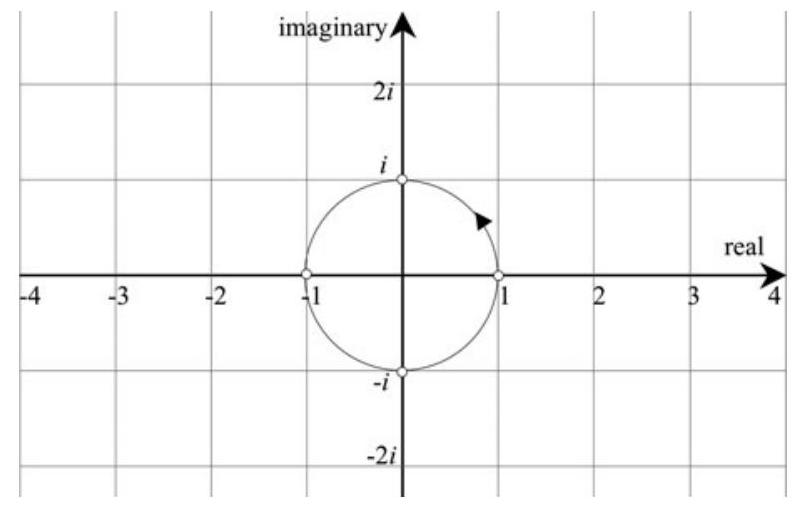
\includegraphics[max width=0.6\textwidth]{2023_01_16_a848224efad29cd66460g-050}
    \caption{带单位圆的复平面}
\end{figure}
它集成了5个重要常数:$0,1,e, \pi$和$i$,以及基本的算术运算:加法,乘法和求幂。

当$\theta=\pi / 2$时,这个公式会产生另一个结果:
$$
e^{i \pi / 2}=\cos \frac{\pi}{2}+i \sin \frac{\pi}{2}=i
$$
因此,\footnote{译者注,和网友讨论,并不止这一种结果,正确的结果应该如此:
\begin{align*}
    \begin{aligned}
        i &=  \cos (\frac{\pi}{2}+2k\pi)+i\sin(\frac{\pi}{2}+2k\pi)\\
        &=e^{i({\pi/2}+2k\pi)},\qquad k\in \mathbb{Z}\\
        i^i &= e^{-(\pi/2+2k\pi)},\qquad k\in \mathbb{Z}\\
    \end{aligned}
\end{align*}

是一个完全的实数的实数幂函数,对应多个值,感谢网友“天津-莲子粥(嵌入式)”。}

$$
\begin{aligned}
i^{i} & =\left(e^{i \pi / 2}\right)^{i} \\
& =e^{i^{2} \pi / 2} \\
& =e^{-\pi / 2} \\
& =0.207879576 \ldots
\end{aligned}
$$
这表明虚数单位自身的幂等于一个实数!\footnote{译者注,参考上一条脚注,应该是一系列实数。}

在第三章中,我们看到虚$i$的幂会产生两个序列$(1,i,-1,-i, 1, \ldots)$和$(1,-i,-1, i, 1, \ldots)$,它们与分别沿逆时针和顺时针方向绕笛卡尔轴旋转时产生的$(x, y,-x,-y, y, x, \ldots)$和$(x,-y,-x, y, x, \ldots)$的模式有着显著的相似之处。这种相似性并非巧合,因为复数属于一个叫做复平面的二维平面,我们现在将描述复平面。

复平面使我们能够可视化复数,横轴记录实数部分,纵轴记录虚数部分,如图4.1所示。该图还显示了一个以单位半径穿过点$1,i,-1,-i$的圆,这是与$i$的幂递增相关的序列。我们可以看到$i^{0}=1, i^{1}=i, i^{2}=-1, i^{3}=-i$和$i^{4}=1$的位置,这表明乘以$i$相当于旋转$90^{\circ}$。为了证明这种旋转效应,图4.2给出了包含四个复数的复平面:
$$
p=2+i, \quad q=-1+2 i, \quad r=-2-i, \quad s=1-2 i
$$
它们之间的距离是$90^{\circ}$。

\begin{figure}[h!]
    \centering
    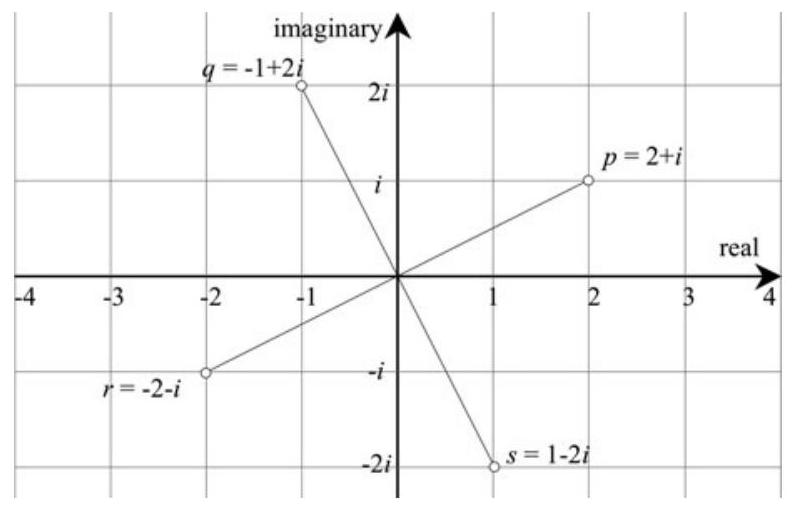
\includegraphics[max width=0.6\textwidth]{2023_01_16_a848224efad29cd66460g-051}
    \caption{标记4个复数的复平面}
\end{figure}

点$p$通过乘以$i$旋转$90^{\circ}$到$q$:
$$
\begin{aligned}
i(2+i) & =2 i+i^{2} \\
& =-1+2 i .
\end{aligned}
$$
点$q$通过乘以$i$旋转$90^{\circ}$到$r$:
$$
\begin{aligned}
i(-1+2 i) & =-i+2 i^{2} \\
& =-2-i .
\end{aligned}
$$
点$r$再乘以$i$旋转$90^{\circ}$到$s$:
$$
\begin{aligned}
i(-2-i) & =-2 i-i^{2} \\
& =1-2 i
\end{aligned}
$$
最后,点$s$乘以$i$被旋转$90^{\circ}$为$p$,:
$$
\begin{aligned}
i(1-2 i) & =i-2 i^{2} \\
& =2+i
\end{aligned}
$$

我们还在第三章中发现,与增加负幂相关的序列:$(1,-i,-1, i, \ldots)$是一个顺时针方向的旋转,这意味着将一个复数除以$i$将它顺时针旋转$90^{\circ}$。然而,我们证明了$i^{-1}=-i$,用$-i$乘以一个复数要比用$i$除以简单得多。所以让我们重复上面的练习来证明这一点。

点$p$乘以$-i$被旋转$-90^{\circ}$到$s$:
$$
\begin{aligned}
-i(2+i) & =-2 i-i^{2} \\
& =1-2 i .
\end{aligned}
$$
点$s$再乘以$-i$旋转$-90^{\circ}$到$r$:
$$
\begin{aligned}
-i(1-2 i) & =-i+2 i^{2} \\
& =-2-i .
\end{aligned}
$$
点$r$再乘以$-i$旋转$-90^{\circ}$到$q$,:
$$
\begin{aligned}
-i(-2-i) & =2 i+i^{2} \\
& =-1+2 i .
\end{aligned}
$$
最后,点$q$乘以$-i$被旋转$-90^{\circ}$为$p$:
$$
\begin{aligned}
-i(-1+2 i) & =i-2 i^{2} \\
& =2+i .
\end{aligned}
$$
因此,将一个复数旋转$\pm 90^{\circ}$,乘以$\pm i$。

在第3章中,我们看到$\sqrt{\pm i}$的根为
$$
\begin{aligned}
& \sqrt{+i}=\pm \frac{\sqrt{2}}{2}(1+i) \\
& \sqrt{-i}=\pm \frac{\sqrt{2}}{2}(1-i)
\end{aligned}
$$
请注意如图4.3所示,每个根之间的距离为$180^{\circ}$,这表明角度与它们的行为有关。例如,$\sqrt{+i}$的正根是$\sqrt{2}/ 2(1+i)$,离实轴为$45^{\circ}$。将这个根乘以它自己,将它$45^{\circ}$旋转到$i$轴。类似地,负根是$-\sqrt{2}/ 2(1+i)$,离实轴为$225^{\circ}$。这个根乘以它自己,将它$225^{\circ}$旋转到$i$轴。$\sqrt{-i}$的根也是如此。

\begin{figure}[h!]
    \centering
    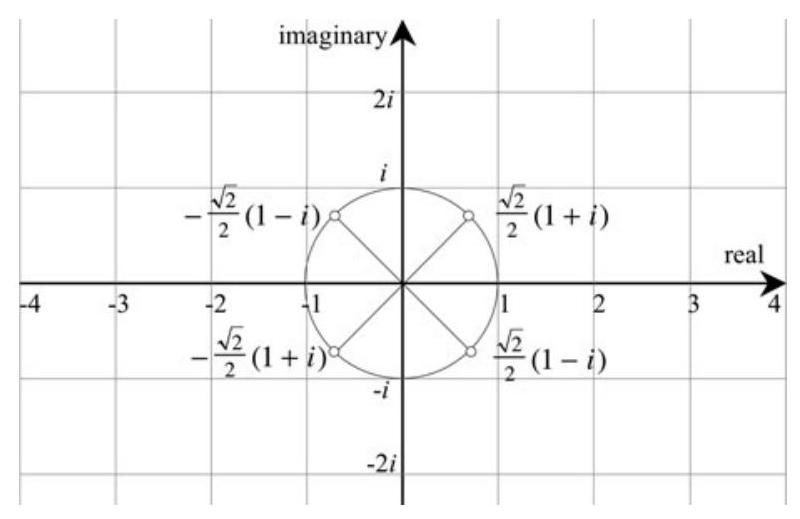
\includegraphics[max width=0.6\textwidth]{2023_01_16_a848224efad29cd66460g-052}
    \caption[short]{$\sqrt{\pm i}$的根}
\end{figure}

这些观察似乎表明,我们可以构造一个能够使另一个复数旋转任意角度的复数。这是真的,我们接下来会讲到。

\section{极坐标表示法}
在复平面上放置一个复数,我们得到极坐标表示,在极坐标表示中,我们从原点到复数形成一条直线,如图4.4所示。这条线的长度是$r$,等于$\sqrt{a^{2}+b^{2}}$,这就是为什么复数的范数是用毕达哥拉斯公式定义的:
\begin{figure}[h!]
    \centering
    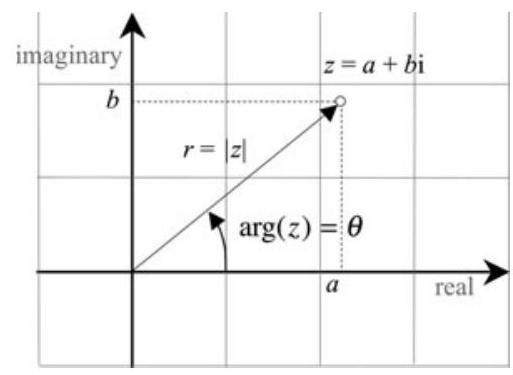
\includegraphics[max width=0.6\textwidth]{2023_01_16_a848224efad29cd66460g-053}
    \caption[short]{复数的极坐标表示
    }
\end{figure}

$$
r=|z|=\sqrt{a^{2}+b^{2}} .
$$
直线与实轴之间的角度$\theta$称为$z$的参数
$$
\arg (z)=\theta
$$
其中
$$
\tan \theta=\frac{b}{a} .
$$
我们计算$\arg (z)$使用
$$
\begin{array}{ll}
\text { 第一象限 } a>0, b>0 & \theta=\arctan (b / a) \\
\text { 第二和第三象限 } a<0 & \theta=\arctan (b / a)+\pi \\
\text { 第四象限 } a>0, b<0 & \theta=\arctan (b / a)+2 \pi .
\end{array}
$$
从图4.4中我们可以看到,z的水平分量是$r \cos \theta$,垂直分量是$r \sin \theta$,这使得我们可以写
$$
\begin{aligned}
z & =a+b i \\
& =r \cos \theta+r i \sin \theta \\
& =r(\cos \theta+i \sin \theta) .
\end{aligned}
$$
如上所述,欧拉的发现之一是关于$e^{\theta}, \sin \theta$和$ cos \theta$幂级数的恒等式:
$$
e^{i \theta}=\cos \theta+i \sin \theta
$$
这允许我们写作
$$
z=r e^{i \theta} .
$$
有了这个发现,我们现在可以用极坐标表示法来重新讨论两个复数的乘积和商。例如,给定下列复数
$$
\begin{aligned}
z & =r e^{i \theta} \\
w & =s e^{i \phi}
\end{aligned}
$$
他们的乘积
$$
\begin{aligned}
z w & =r s e^{i \theta} e^{i \phi} \\
& =r s e^{i(\theta+\phi)} \\
& =r s[\cos (\theta+\phi)+i \sin (\theta+\phi)]
\end{aligned}
$$
所以两个复数的乘积会产生第三个有范数的复数
$$
|z w|=r s
$$
且参数
$$
\arg (z w)=\theta+\phi
$$
这里两个角直接相加了。

接下来,除法:
$$
\begin{aligned}
\frac{z}{w} & =\frac{r e^{i \theta}}{s e^{i \phi}} \\
& =\frac{r}{s} e^{i(\theta-\phi)} \\
& =\frac{r}{s}[\cos (\theta-\phi)+i \sin (\theta-\phi)]
\end{aligned}
$$
其中,范数是
$$
\left|\frac{z}{w}\right|=\frac{r}{s}
$$
且参数为
$$
\arg (z / w)=\theta-\phi
$$
这里是两个角度相减了。

让我们用一个例子来应用这些公式。图$4.5$显示了两个复数
$$
\begin{gathered}
z=2+2 i \\
w=-1+i
\end{gathered}
$$
在极坐标形式里面是
$$
\begin{aligned}
z & =2 \sqrt{2}\left(\cos 45^{\circ}+i \sin 45^{\circ}\right)=2 \sqrt{2} e^{i \pi / 4} \\
w & =\sqrt{2}\left(\cos 135^{\circ}+i \sin 135^{\circ}\right)=\sqrt{2} e^{i 3 \pi / 4} .
\end{aligned}
$$
用普通的复代数,乘积$z w$是
$$
z w=(2+2 i)(-1+i)=-4
$$
\begin{figure}[h!]
    \centering
    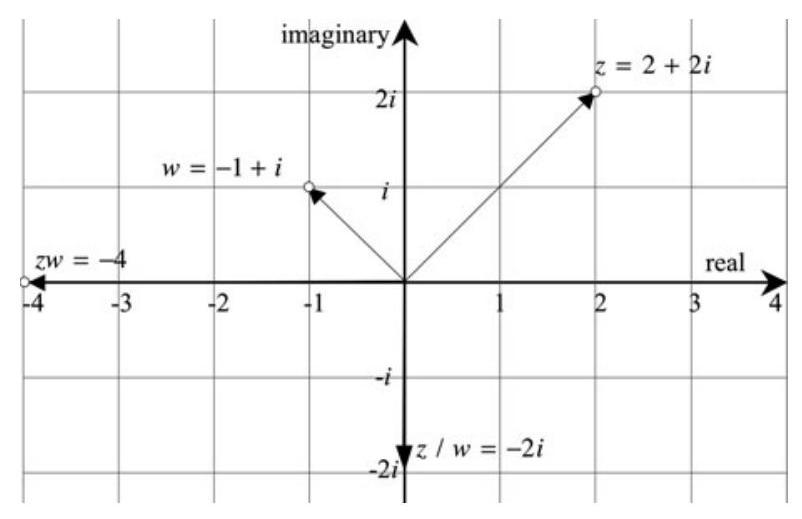
\includegraphics[max width=0.6\textwidth]{2023_01_16_a848224efad29cd66460g-055}
    \caption[short]{两个复数的乘积}
\end{figure}
用极坐标形式是:
$$
\begin{aligned}
|z w| & =2 \sqrt{2} \sqrt{2}=4 \\
\arg (z w) & =45^{\circ}+135^{\circ}=180^{\circ}
\end{aligned}
$$
这里编码为$-4$。

现在让我们用普通的复代数和极坐标形式来计算商$z / w$。
$$
\begin{aligned}
\frac{z}{w} & =\frac{(2+2 i)}{(-1+i)} \frac{(-1-i)}{(-1-i)} \\
& =\frac{-2-2 i-2 i-2 i^{2}}{1+1} \\
& =-2 i
\end{aligned}
$$
接下来,使用极坐标形式:
$$
\begin{aligned}
|z / w| & =\frac{2 \sqrt{2}}{\sqrt{2}}=2 \\
\arg (z / w) & =45^{\circ}-135^{\circ}=-90^{\circ}
\end{aligned}
$$
这编码复数$-2 i$。这些结果如图4.5所示。

我们还可以使用欧拉公式计算$\sqrt{i}$ ,如下所示
$$
e^{i \theta}=\cos \theta+i \sin \theta
$$
将$\theta=\pi / 2$代入
$$
e^{i \pi / 2}=\cos \frac{\pi}{2}+i \sin \frac{\pi}{2}=i
$$
两边同时开根号,得到
$$
\begin{aligned}
e^{i \pi / 4} & =\pm \sqrt{i} \\
\cos \frac{\pi}{4}+i \sin \frac{\pi}{4} & =\pm \sqrt{i} \\
\pm \frac{\sqrt{2}}{2}(1+i) & =\pm \sqrt{i}
\end{aligned}
$$
为了找到$\sqrt{-i}$,我们代入$\theta=-\pi / 2$:
$$
\begin{aligned}
e^{-i \pi / 2} & =\cos \left(-\frac{\pi}{2}\right)+i \sin \left(-\frac{\pi}{2}\right)=-i \\
& =\cos \left(\frac{\pi}{2}\right)-i \sin \left(\frac{\pi}{2}\right)=-i
\end{aligned}
$$
两边同时开根号,得到
$$
\begin{aligned}
e^{-i \pi / 4} & =\pm \sqrt{-i} \\
\cos \left(\frac{\pi}{4}\right)-i \sin \left(\frac{\pi}{4}\right) & =\pm \sqrt{-i} \\
\pm \frac{\sqrt{2}}{2}(1-i) & =\pm \sqrt{-i}
\end{aligned}
$$
用类似的方法可以找到更高次的根。

\section{转子}
极坐标形式说明了这样一个事实:范数为$r$的复数$z=r e^{i \theta}$与范数为$s$的复数$w=s e^{i \phi}$相乘,就得到了第三个范数为$r s$的复数。因此,为了避免缩放$z, w$必须有一个范数单位$1$。在这种情况下,$w$充当转子。例如,用$4+5 i$乘以$1+0 i$,它就没有缩放和旋转。然而,用$4+5 i$乘以$0+i$将它旋转$90^{\circ}$而不进行任何缩放。

因此,要将$2+2 i$旋转$45^{\circ}$,我们必须将它乘以$e^{i \pi / 4}$:
$$
\begin{aligned}
e^{i \pi / 4} & =\cos 45^{\circ}+i \sin 45^{\circ}=\frac{\sqrt{2}}{2}(1+i) \\
\frac{\sqrt{2}}{2}(1+i)(2+2 i) & =\frac{\sqrt{2}}{2} 4 i \\
& =2 \sqrt{2} i .
\end{aligned}
$$
因此$e^{i \theta}$将任何复数旋转一个角度$\theta$。

要使复数$x+y i$旋转一个角度$\theta$,我们可以将它乘以转子$\cos \theta+i \sin \theta$:
$$
\begin{aligned}
x^{\prime}+y^{\prime} i & =(\cos \theta+i \sin \theta)(x+y i) \\
& =x \cos \theta-y \sin \theta+i(x \sin \theta+y \cos \theta)
\end{aligned}
$$
矩阵形式是:
$$
\left[\begin{array}{cc}
x^{\prime} & -y^{\prime} \\
y^{\prime} & x^{\prime}
\end{array}\right]=\left[\begin{array}{cc}
\cos \theta & -\sin \theta \\
\sin \theta & \cos \theta
\end{array}\right]\left[\begin{array}{cc}
x & -y \\
y & x
\end{array}\right] .
$$
在继续之前,让我们考虑转子的复共轭对旋转方向的影响,我们可以通过将$x+y i$乘以转子$\cos \theta -i \sin \theta$来实现
$$
\begin{aligned}
x^{\prime}+y^{\prime} i & =(\cos \theta-i \sin \theta)(x+y i) \\
& =x \cos \theta+y \sin \theta-i(x \sin \theta+y \cos \theta)
\end{aligned}
$$
矩阵形式是
$$
\left[\begin{array}{cc}
x^{\prime} & -y^{\prime} \\
y^{\prime} & x^{\prime}
\end{array}\right]=\left[\begin{array}{cc}
\cos \theta & \sin \theta \\
-\sin \theta & \cos \theta
\end{array}\right]\left[\begin{array}{cc}
x & -y \\
y & x
\end{array}\right]
$$
也就是绕原点旋转$-\theta$。

因此,我们定义一个转子$\mathbf{R}_{\theta}$和它的共轭$\mathbf{R}_{\theta}^{\dagger}$为
$$
\begin{aligned}
& \mathbf{R}_{\theta}=\cos \theta+i \sin \theta \\
& \mathbf{R}_{\theta}^{\dagger}=\cos \theta-i \sin \theta
\end{aligned}
$$
其中$\mathbf {R} _{\theta}$旋转$+ \theta$,和$\mathbf{R}_{\theta}^{\dagger}$旋转$- \theta$。注意,使用了匕首$\dagger$符号。

\section{总结}
在本章中,我们发现了用复平面来表示复数的图形化解释。欧拉公式$e^{i \theta}=\cos \theta+i \sin \theta$允许我们将复数表示为$e$的虚数次幂,从而使我们可以轻松地计算乘积和商。总的来说,这些想法把我们引向了转子的想法,它将使用四元数来开发。

\subsection{运算符总结}
\subsubsection*{复数}
$$
\begin{aligned}
z & =a+b i \\
|z| & =\sqrt{a^{2}+b^{2}}
\end{aligned}
$$

\subsubsection*{极坐标表示}

$$
\begin{aligned}
z & =r e^{i \theta} \\
z & =r(\cos \theta+i \sin \theta) \\
r & =|z| \\
\tan \theta & =b / a \\
\theta & =\arg (z)
\end{aligned}
$$

\begin{align*}
    \begin{aligned}
        &\text{第一象限  } a>0, b>0 && \theta=\arctan (b / a)\\
        &\text{第二和第三象限  } a<0 && \theta=\arctan (b / a)+\pi\\
        &\text{第四象限  } a>0, b<0 && \theta=\arctan (b / a)+2 \pi.
    \end{aligned}
\end{align*}


\subsubsection*{乘积}
$$
\begin{aligned}
z & =r e^{i \theta} \\
w & =s e^{i \phi} \\
z w & =r s e^{i(\theta+\phi)} \\
& =r s[\cos (\theta+\phi)+i \sin (\theta+\phi)]
\end{aligned}
$$

\subsubsection*{商}
$$
\begin{aligned}
\frac{z}{w} & =\frac{r}{s} e^{i(\theta-\phi)} \\
& =\frac{r}{s}[\cos (\theta-\phi)+i \sin (\theta-\phi)]
\end{aligned}
$$

\subsubsection*{转子}
$$
\begin{aligned}
& \mathbf{R}_{\theta}=\cos \theta+i \sin \theta \\
& \mathbf{R}_{\theta}^{\dagger}=\cos \theta-i \sin \theta
\end{aligned}
$$

\section{样例}
下面是一些进一步使用上述思想的示例。在某些情况下,包括测试来确认结果。
\begin{example}
    
    从$1+2 i$开始,将得到的复数乘以$i$四次,并将结果绘制在复平面上。
    
    点$p$通过乘以$i$旋转$90^{\circ}$到$q$:
    $$
    \begin{aligned}
    i(1+2 i) & =i+2 i^{2} \\
    & =-2+i .
    \end{aligned}
    $$
    
    点$q$通过乘以$i$旋转$90^{\circ}$到$r$:
    $$
    \begin{aligned}
    i(-2+i) & =-2 i+i^{2} \\
    & =-1-2 i
    \end{aligned}
    $$
    
    点$r$再乘以$i$旋转$90^{\circ}$到$s$:
    $$
    \begin{aligned}
    i(-1-2 i) & =-i-2 i^{2} \\
    & =2-i .
    \end{aligned}
    $$
    
    最后,点$s$乘以$i$被旋转$90^{\circ}$为$p$:
    $$
    \begin{aligned}
    i(2-i) & =2 i-i^{2} \\
    & =2+i .
    \end{aligned}
    $$
    
    图$4.6$显示了四个被$90^{\circ}$隔开的复数。
    \begin{figure}[h!]
        \centering
        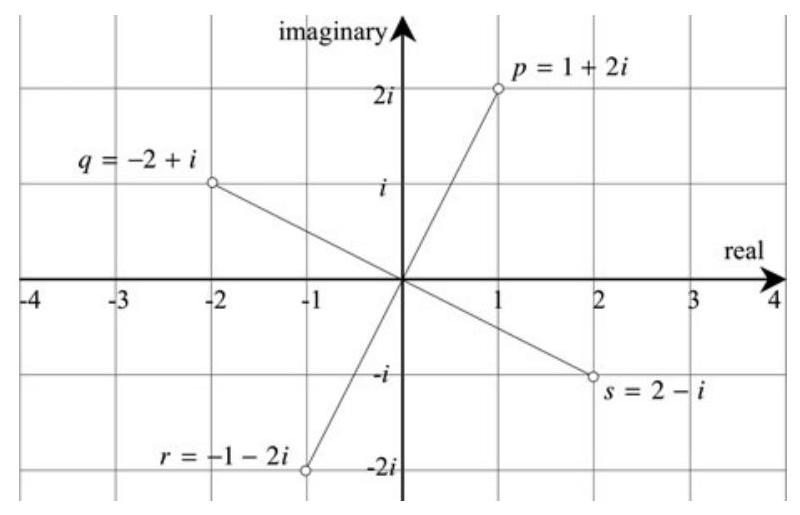
\includegraphics[max width=0.6\textwidth]{2023_01_16_a848224efad29cd66460g-059}
        \caption{有四个复数的复平面}
    \end{figure}
\end{example}

\begin{example}
    用极坐标形式计算乘积$ zw $和商$z / w$。
    $$
    \begin{gathered}
    z=3+3 i \\
    w=-1-i
    \end{gathered}
    $$
    
    乘积:
    $$
    \begin{aligned}
    z & =3 \sqrt{2}\left(\cos 45^{\circ}+i \sin 45^{\circ}\right)=3 \sqrt{2} e^{i \pi / 4} \\
    w & =\sqrt{2}\left(\cos 225^{\circ}+i \sin 225^{\circ}\right)=\sqrt{2} e^{i 5 \pi / 4} \\
    |z w| & =3 \sqrt{2} \sqrt{2}=6 \\
    \arg (z w) & =45^{\circ}+225^{\circ}=270^{\circ}
    \end{aligned}
    $$
    这编码复数$-6 i$。
    
    测试:使用普通的复代数,乘积$ zw $为
    $$
    z w=(3+3 i)(-1-i)=-6 i .
    $$
    
    商:
    $$
    \begin{aligned}
    |z| & =3 \sqrt{2} \\
    |w| & =\sqrt{2} \\
    |z / w| & =3 \sqrt{2} / \sqrt{2}=3 \\
    \arg (z / w) & =45^{\circ}-225^{\circ}=180^{\circ}
    \end{aligned}
    $$
    这编码复数$-3$.
    
    测试:使用普通的复代数,乘积$ z/w $为
    $$
    \begin{aligned}
    \frac{z}{w} & =\frac{(3+3 i)}{(-1-i)} \frac{(-1+i)}{(-1+i)} \\
    & =\frac{-6}{2} \\
    & =-3
    \end{aligned}
    $$
    
    并且符合极坐标形式。
\end{example}

\begin{example}
    设计一个转子,将一个复数旋转$30^{\circ}$而不缩放。
    
    这样开始
    $$
    e^{i \theta}=\cos \theta+i \sin \theta
    $$
    
    令 $\theta=30^{\circ}=\pi / 6$
    $$
    \begin{aligned}
    e^{i \pi / 6} & =\cos 30^{\circ}+i \sin 30^{\circ} \\
    & =\frac{\sqrt{3}}{2}+i \frac{1}{2} \\
    & =\frac{1}{2}(\sqrt{3}+i) .
    \end{aligned}
    $$
    
    测试:让我们用这个转子将$1+0 i$旋转三次到$i$。
    $$
    \begin{aligned}
    \frac{1}{2}(\sqrt{3}+i) \frac{1}{2}(\sqrt{3}+i) \frac{1}{2}(\sqrt{3}+i) 1 & =\frac{1}{8}(\sqrt{3}+i)(\sqrt{3}+i)(\sqrt{3}+i) \\
    & =\frac{1}{8}(2+2 \sqrt{3} i)(\sqrt{3}+i) \\
    & =\frac{1}{8}(2 \sqrt{3}-2 \sqrt{3}+2 i+6 i) \\
    & =i
    \end{aligned}
    $$
\end{example}

\begin{example}
    设计一个转子,将一个复数旋转$-60^{\circ}$而不缩放。
    
    这样开始
    $$
    e^{i \theta}=\cos \theta+i \sin \theta
    $$
    
    令 $\theta=-60^{\circ}=-\pi / 3$
    
    $$
    \begin{aligned}
    e^{-i \pi / 3} & =\cos \left(-60^{\circ}\right)+i \sin \left(-60^{\circ}\right) \\
    & =\frac{1}{2}-\frac{\sqrt{3}}{2} i \\
    & =\frac{1}{2}(1-\sqrt{3} i)
    \end{aligned}
    $$
\end{example}

%\include{num_pro}
%\include{mod_trans}



\clearpage
\end{CJK}
\end{document}